\chapter{\textit{The GCD Cascade: Cracking Numbers Open with Pythagorean Channels}}
\label{ch13}



\bigskip


\section{The Eavesdropper's Puzzle}

I am thinking of two secret prime numbers, $p$ and $q$. I will not tell you either one. But I will tell you that their product is $p \times q = 4{,}579$, and that I have found four integers $a, b, c, d$ satisfying
\index{prime number}

\[
a^2 + b^2 + c^2 = d^2
\]

with $d = pq = 4{,}579$. Here is the quadruple: $(390, 1{,}738, 4{,}122, 4{,}579)$. From this quadruple alone --- without trial division, without a sieve, without any brute-force search --- can you recover $p$ and $q$?

The answer, against all intuition, is \textit{yes}. And the method is the subject of this chapter.

What makes this trick work is a network of hidden relationships --- \textit{channels} --- woven into every Pythagorean quadruple. Each channel carries partial information about the hypotenuse's factors, like an encrypted broadcast. Intercepting a single channel may reveal nothing. But cross-referencing two or three channels, using the oldest and most elementary tool in number theory --- the greatest common divisor --- sets off a \textit{cascade} of deductions that tears the composite apart. The GCD cascade is not a modern algorithm dressed in ancient clothing. It is ancient arithmetic performing a modern miracle.
\index{greatest common divisor}
\index{GCD cascade}
\index{Pythagorean quadruple}

\begin{figure}[htbp]
\centering
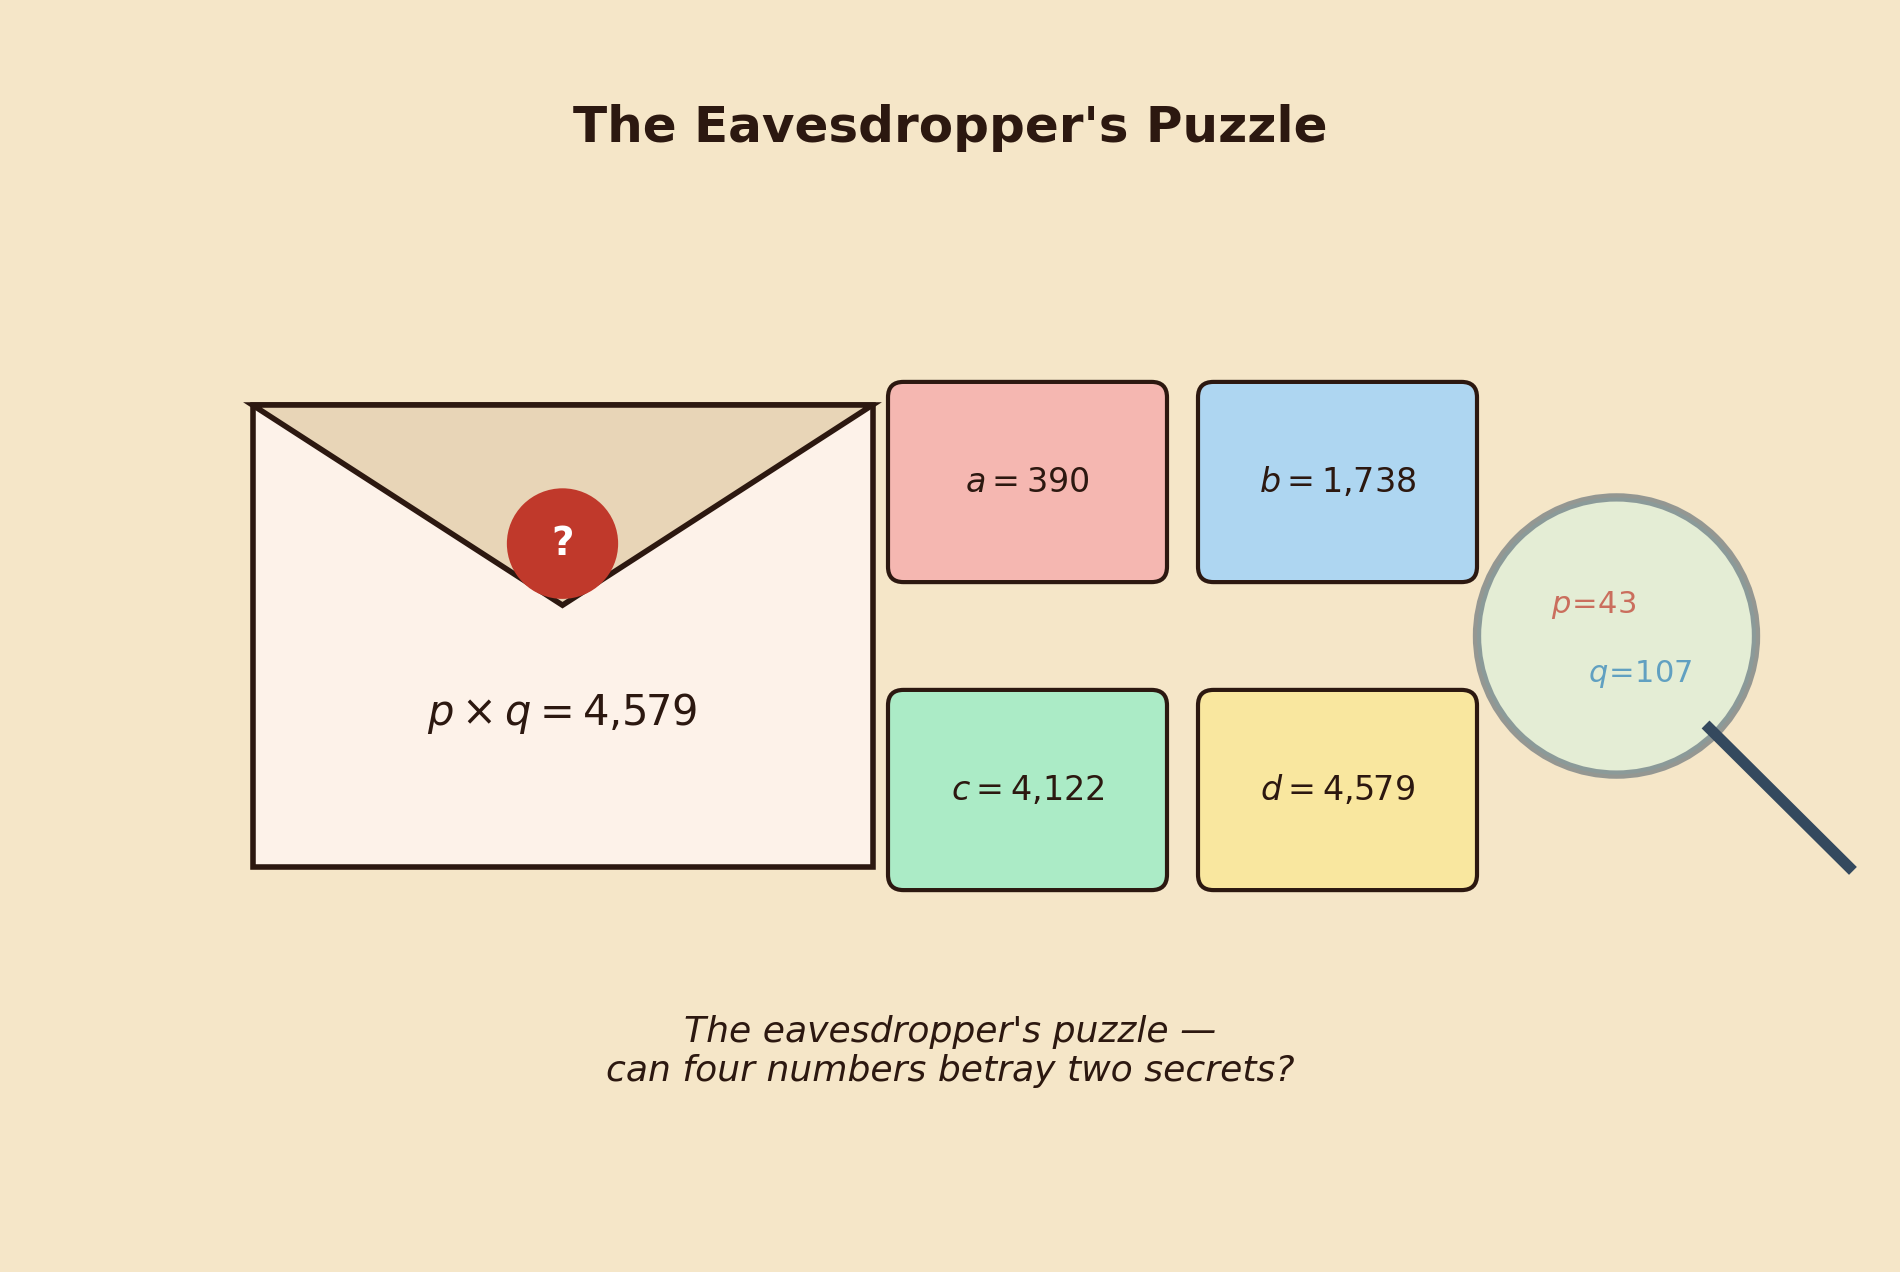
\includegraphics[width=0.82\textwidth]{../Chapter13/images/fig01_eavesdropper.png}
\caption{A sealed envelope labeled "$p \times q = 4{,}579$" sits on a desk beside four numbered cards showing $a = 390$, $b = 1{,}738$, $c = 4{,}122$, $d = 4{,}579$. A magnifying glass hovers over the cards,\ldots}
\end{figure}


\bigskip


\section{Three Channels, One Tower}

Every Pythagorean quadruple $(a, b, c, d)$ satisfying $a^2 + b^2 + c^2 = d^2$ conceals three natural sub-structures, which I shall call \textit{channels}. Define them as the pairwise sums of squared legs:

\[
\mathrm{Ch}_{ab} = a^2 + b^2, \qquad \mathrm{Ch}_{ac} = a^2 + c^2, \qquad \mathrm{Ch}_{bc} = b^2 + c^2.
\]

Each channel has a twin identity. Since $a^2 + b^2 + c^2 = d^2$, we may subtract one squared leg from both sides and discover that every channel is also a \textit{difference of squares} involving the hypotenuse:
\index{difference of squares}

\[
\mathrm{Ch}_{ab} = d^2 - c^2, \qquad \mathrm{Ch}_{ac} = d^2 - b^2, \qquad \mathrm{Ch}_{bc} = d^2 - a^2.
\]

And each difference of squares factors beautifully:

\[
\mathrm{Ch}_{ab} = (d - c)(d + c), \qquad \mathrm{Ch}_{ac} = (d - b)(d + b), \qquad \mathrm{Ch}_{bc} = (d - a)(d + a).
\]

The three channels are like three radio stations broadcasting from the same tower. Each carries a different signal, but together they tell you exactly how tall the tower is. How? Add them up:

\[
\mathrm{Ch}_{ab} + \mathrm{Ch}_{ac} + \mathrm{Ch}_{bc} = (a^2 + b^2) + (a^2 + c^2) + (b^2 + c^2) = 2(a^2 + b^2 + c^2) = 2d^2.
\]

This is the \textbf{Channel Sum Law}: the three channels always sum to exactly twice the squared hypotenuse. It is a small miracle of cancellation --- each of $a^2$, $b^2$, $c^2$ appears in exactly two channels, so the sum double-counts every squared leg and recovers $2d^2$. Simple, inevitable, and surprisingly powerful.

\begin{figure}[htbp]
\centering
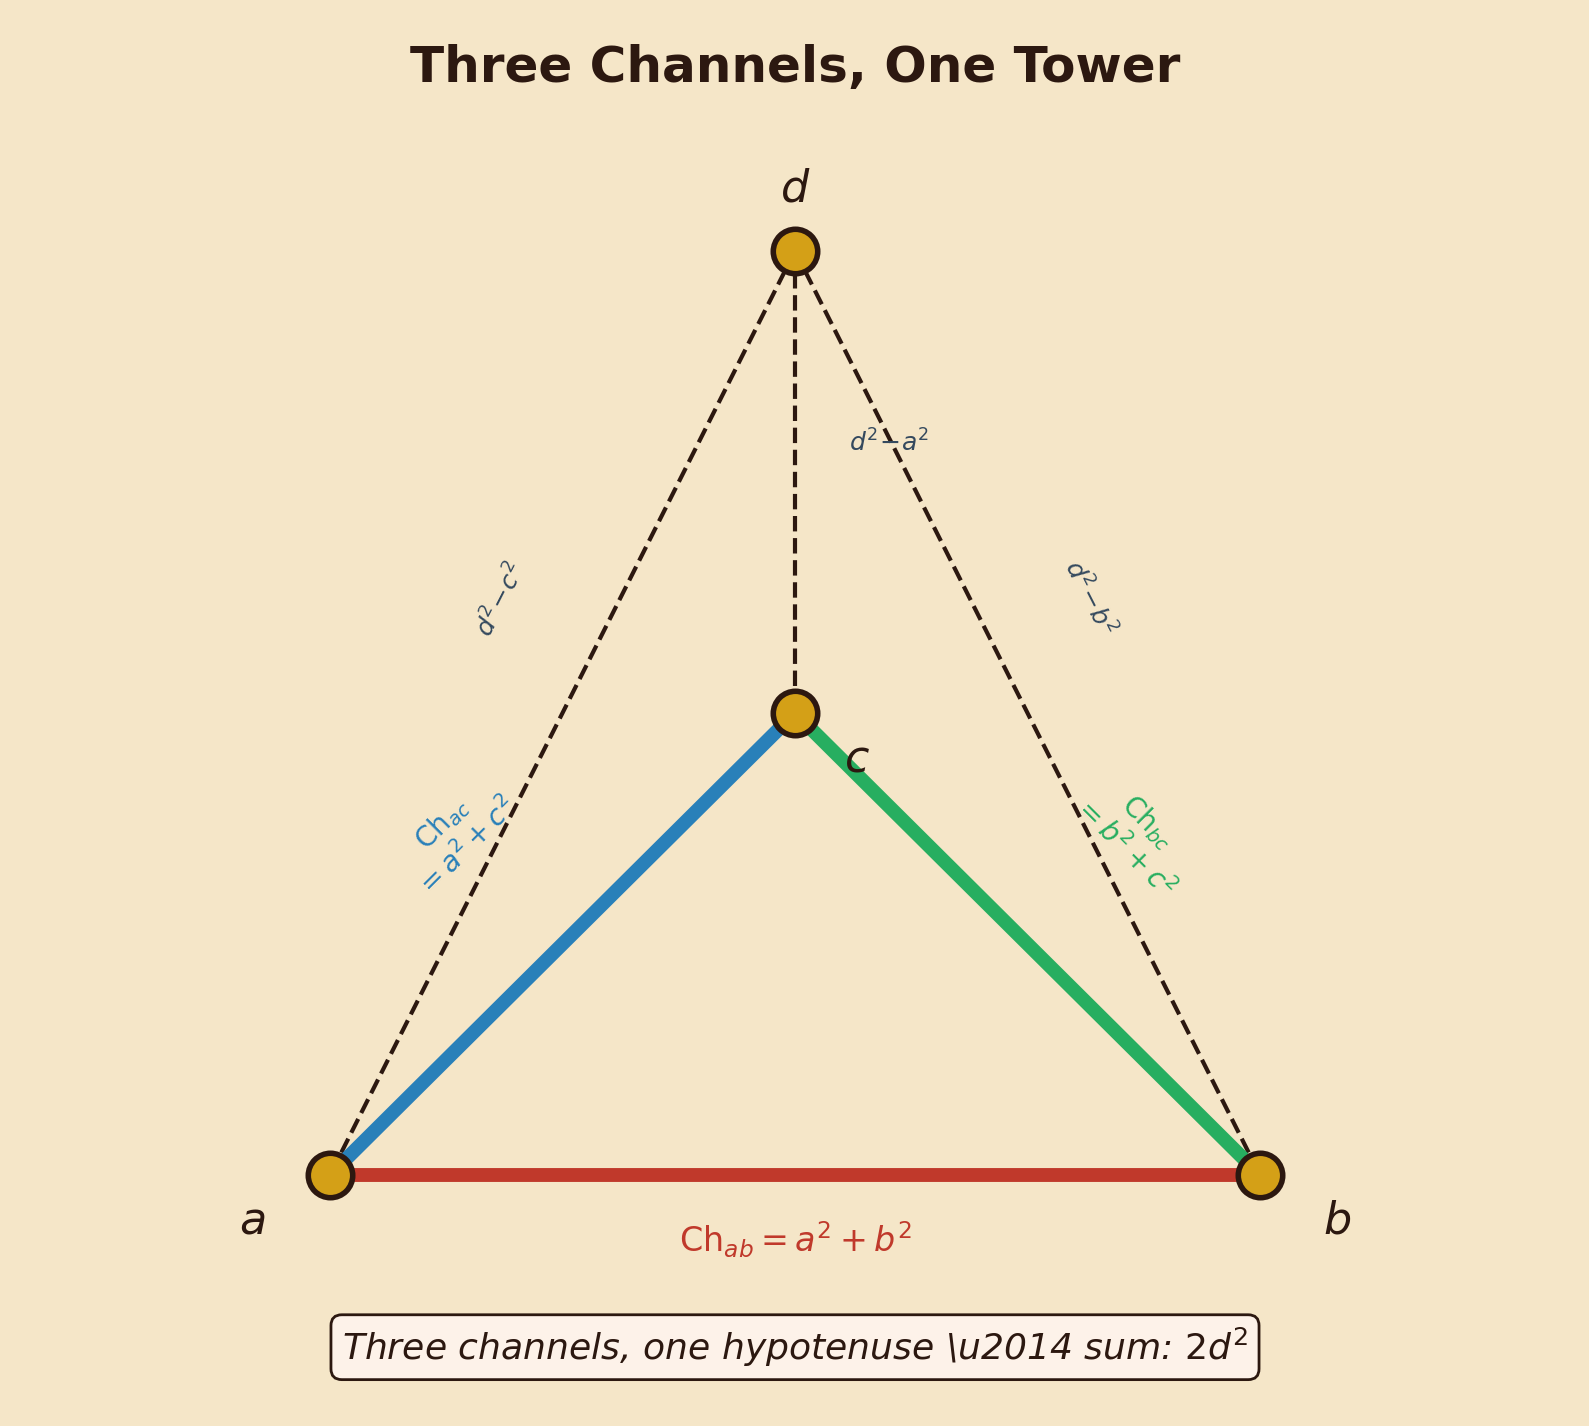
\includegraphics[width=0.82\textwidth]{../Chapter13/images/fig02_channel_tetrahedron.png}
\caption{A tetrahedron whose four vertices are labeled $a$, $b$, $c$, $d$. The three edges connecting pairs among $\{a, b, c\}$ are drawn as thick colored cables --- red for $\mathrm{Ch}_{ab} = a^2 + b^2$, blue\ldots}
\end{figure}


\bigskip


\section{Cross-Channel Eavesdropping}

Suppose you are an intelligence analyst intercepting two encrypted messages from different channels. Individually, each message is opaque. But by comparing what they share --- their greatest common divisor --- you can deduce information that neither channel reveals alone.

Here is the mathematical reality behind the metaphor. If a number $g$ divides both $\mathrm{Ch}_{ab} = a^2 + b^2$ and $\mathrm{Ch}_{ac} = a^2 + c^2$, then $g$ must also divide their difference:

\[
g \mid (a^2 + b^2) \;\;\text{and}\;\; g \mid (a^2 + c^2) \quad \Longrightarrow \quad g \mid (b^2 - c^2).
\]

This is nothing but the subtraction principle for divisibility --- ancient, elementary, and devastating. It extends: if $g$ divides \textit{all three} channels, then $g$ divides every pairwise squared difference $a^2 - b^2$, $a^2 - c^2$, and $b^2 - c^2$.

But there is a deeper prize. Notice the elegant identity

\[
2a^2 = \mathrm{Ch}_{ab} + \mathrm{Ch}_{ac} - \mathrm{Ch}_{bc},
\]

which you can verify by expanding the right-hand side: $(a^2 + b^2) + (a^2 + c^2) - (b^2 + c^2) = 2a^2$. Symmetrically, $2b^2 = \mathrm{Ch}_{ab} + \mathrm{Ch}_{bc} - \mathrm{Ch}_{ac}$ and $2c^2 = \mathrm{Ch}_{ac} + \mathrm{Ch}_{bc} - \mathrm{Ch}_{ab}$. So if $g$ divides all three channels, then $g$ divides $2a^2$, $2b^2$, and $2c^2$. The three-channel constraint is strikingly similar to how a GPS receiver uses three satellite signals to triangulate a position --- except here we are triangulating the \textit{factors} of a number.

\begin{figure}[htbp]
\centering
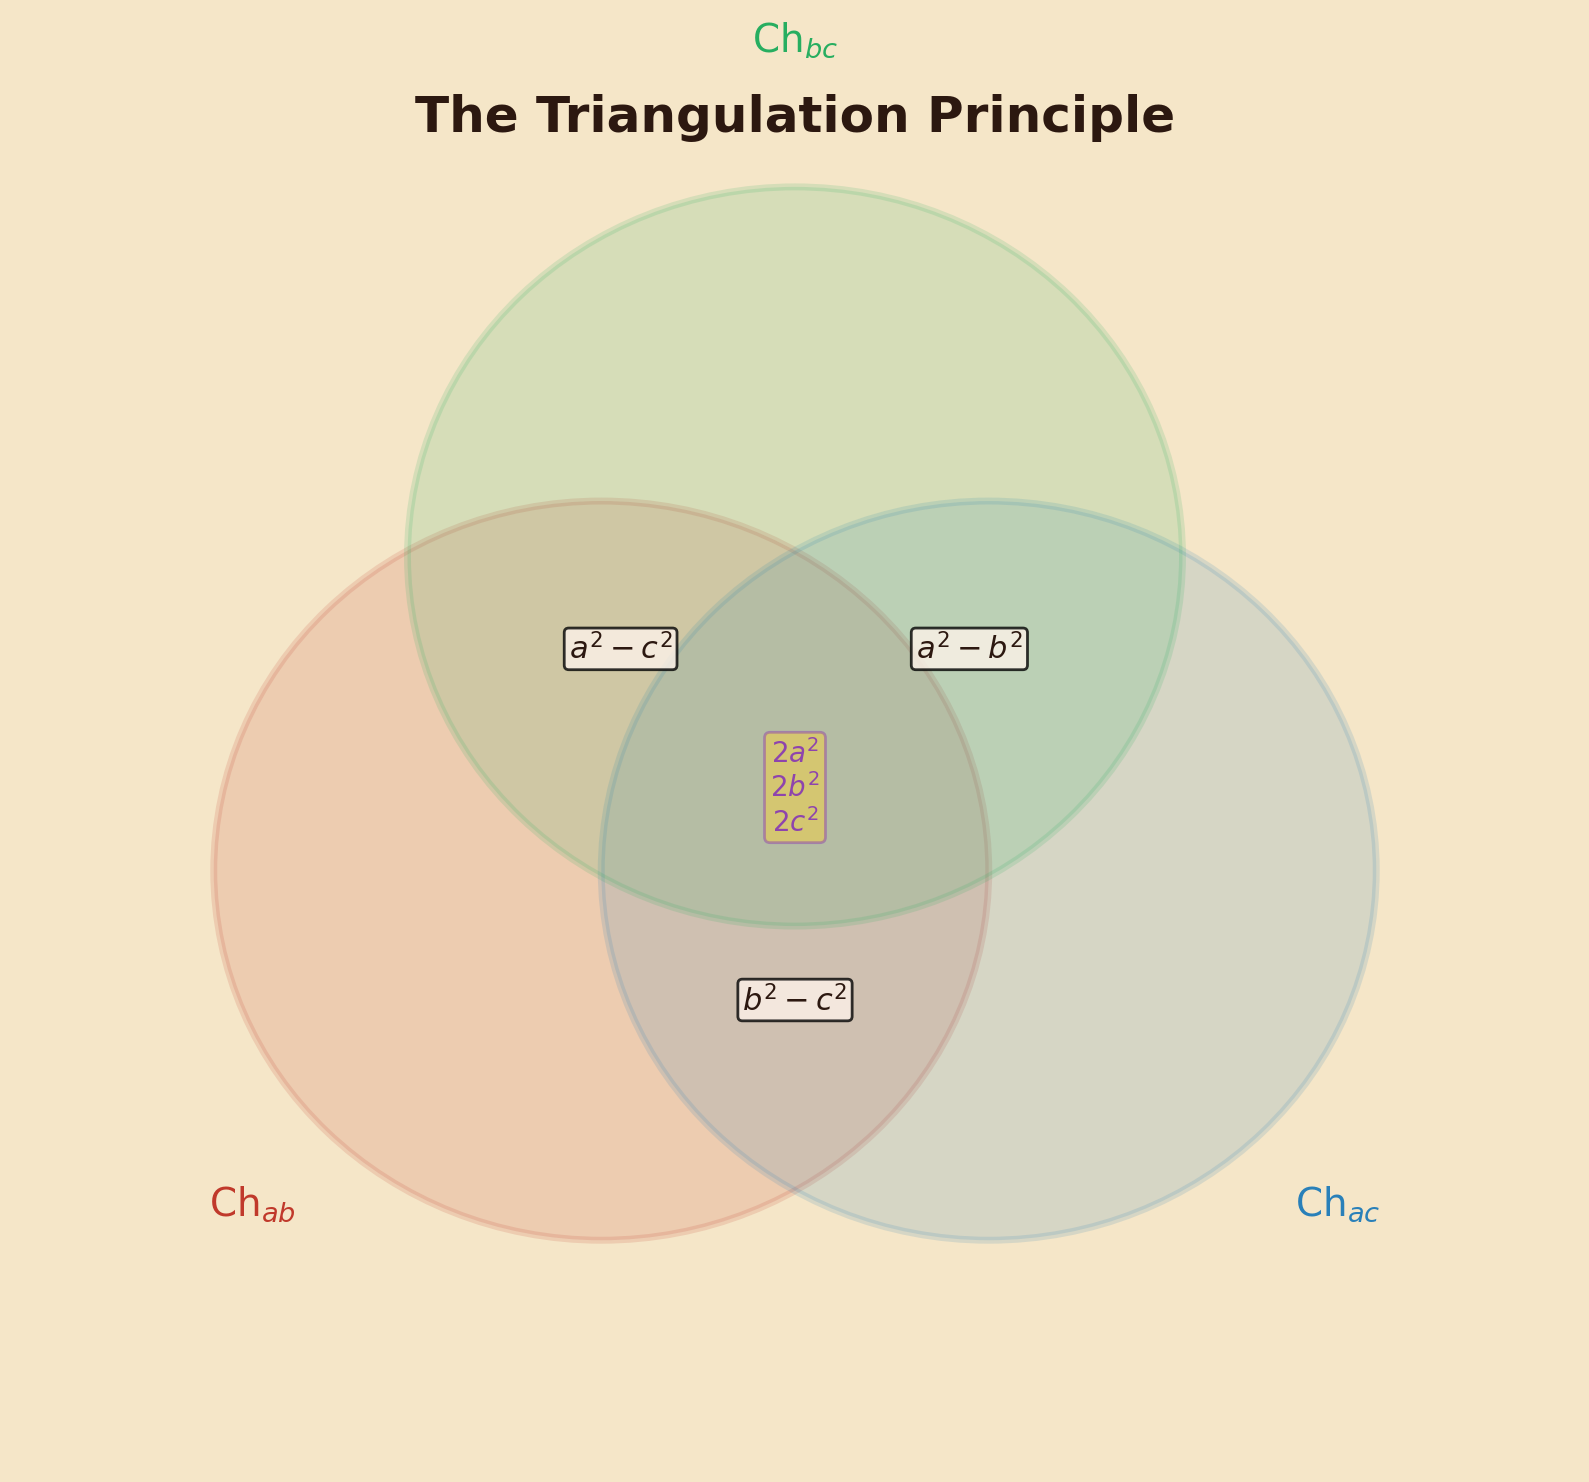
\includegraphics[width=0.82\textwidth]{../Chapter13/images/fig03_triangulation_venn.png}
\caption{A Venn diagram with three large overlapping circles labeled $\mathrm{Ch}_{ab}$, $\mathrm{Ch}_{ac}$, $\mathrm{Ch}_{bc}$ in red, blue, and green respectively. In the pairwise intersection of the red\ldots}
\end{figure}


\bigskip


\section{The Prime Cascade}

Here is a number: $b^2 - c^2 = 1{,}056$. I also know that $b^2 - c^2 = (b - c)(b + c)$. A prime $p$ divides $1{,}056$. Without knowing $b$ or $c$ individually, can you guarantee that $p$ divides either $b - c$ or $b + c$?

You can --- and the guarantee is as old as Euclid. Book VII of the \textit{Elements}, Proposition 30, states that if a prime divides a product, it must divide one of the factors. In modern dress:

\[
p \mid (b - c)(b + c) \quad \Longrightarrow \quad p \mid (b - c) \;\;\text{or}\;\; p \mid (b + c).
\]

This is Euclid's lemma, and it turns the cross-channel theorem into a \textit{cascade}. Suppose we know that a prime $p$ divides both $\mathrm{Ch}_{ab}$ and $\mathrm{Ch}_{ac}$. By the subtraction principle, $p \mid (b^2 - c^2)$. By Euclid's lemma, $p \mid (b - c)$ or $p \mid (b + c)$. A single prime, detected in one channel subtraction, propagates into sums and differences of the raw components $a$, $b$, $c$. The dominos fall: once $p$ divides $b - c$, say, then from $p \mid (a^2 + b^2)$ we can deduce further relationships between $p$ and the components. The cascade has begun, and it does not stop until the factor is fully exposed.

Euclid stated his lemma around 300 BCE. For more than two millennia, mathematicians regarded it as a tidy observation about primes. They had no idea it was a \textit{factoring engine}.
\index{factoring}

\begin{figure}[htbp]
\centering
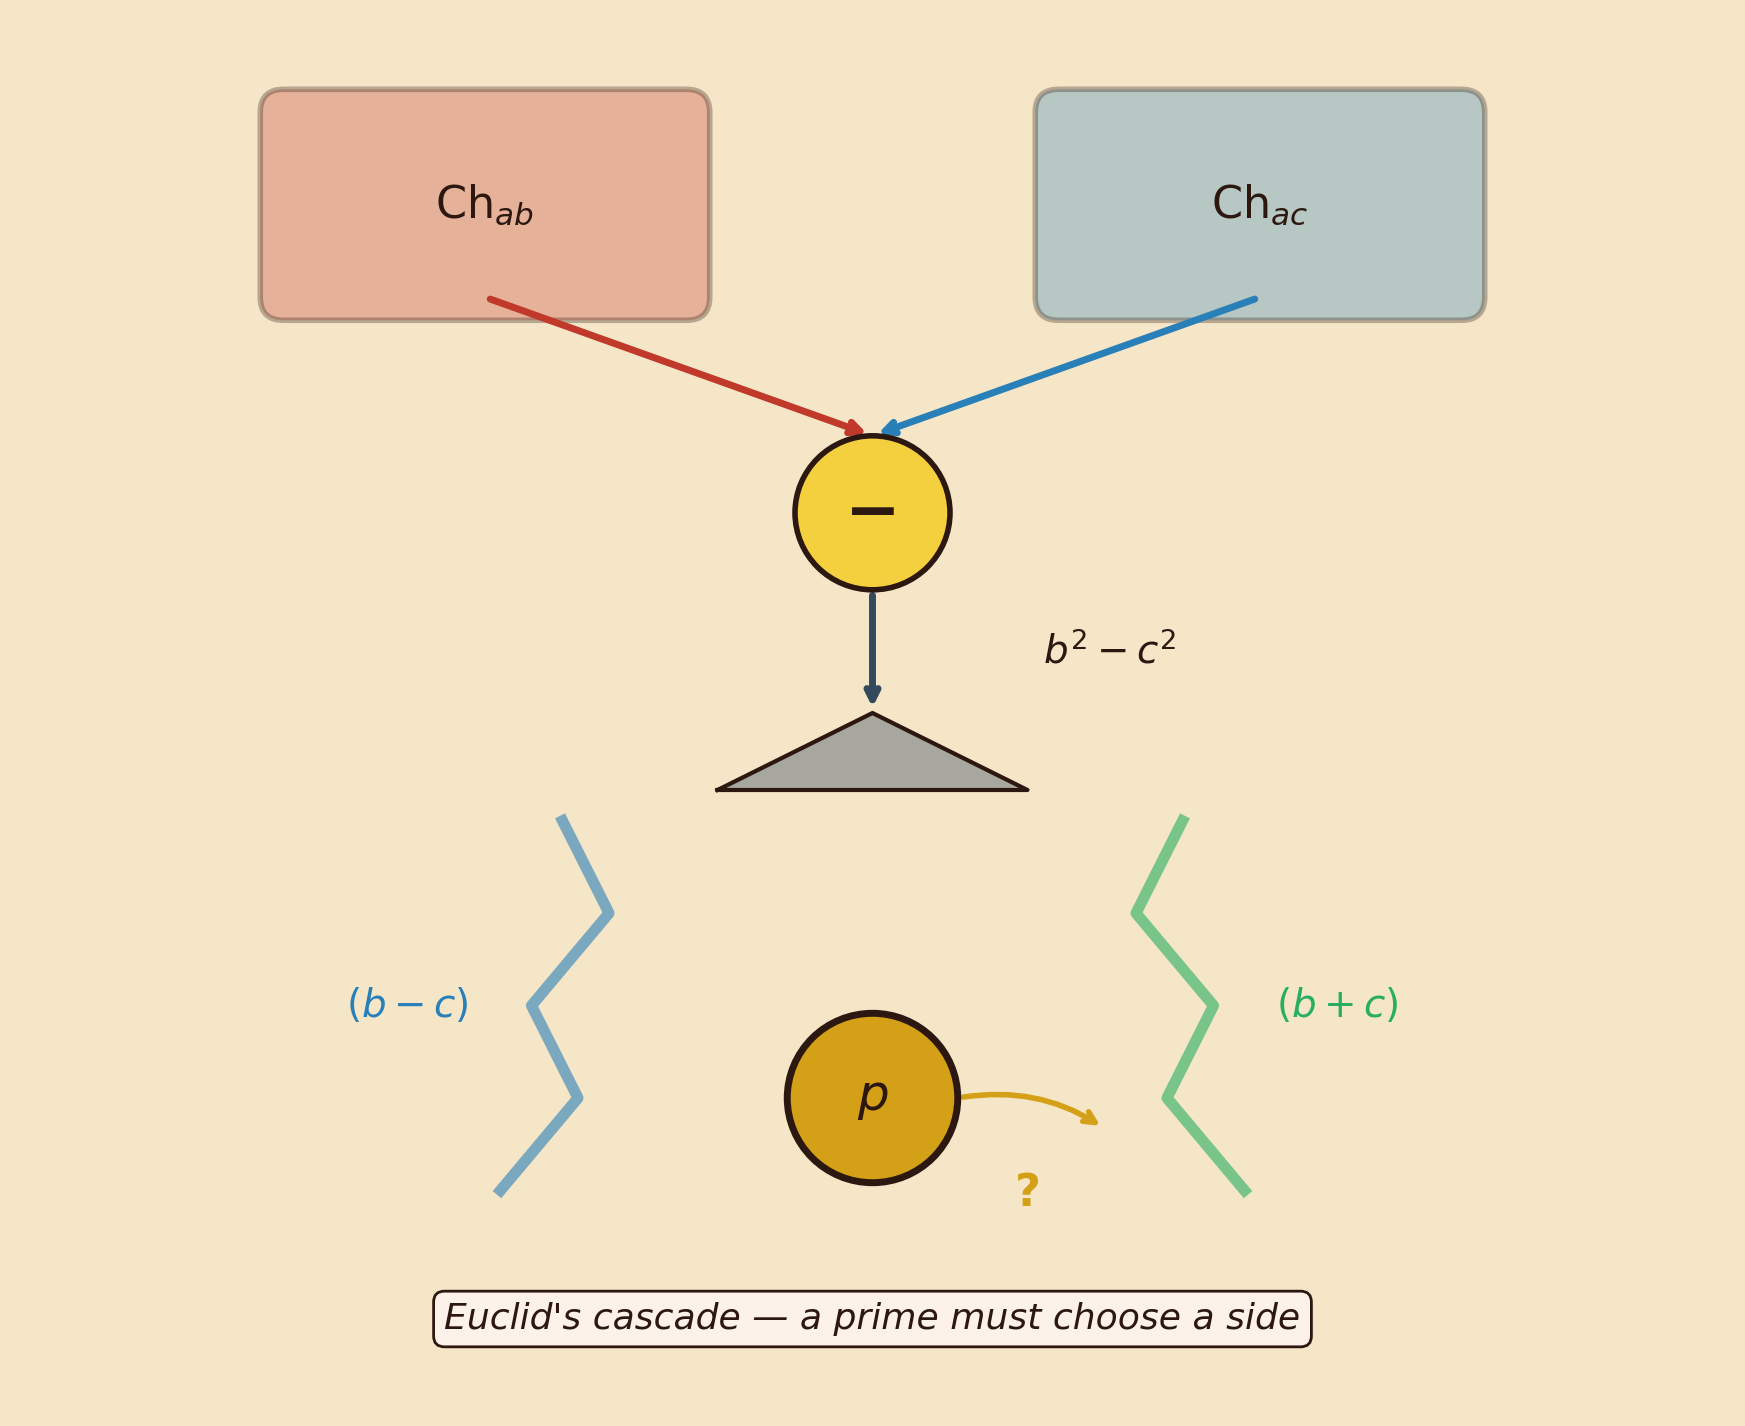
\includegraphics[width=0.82\textwidth]{../Chapter13/images/fig04_cascade_waterfall.png}
\caption{A "waterfall" or cascade diagram. At the top, two rectangular boxes labeled $\mathrm{Ch}_{ab}$ and $\mathrm{Ch}_{ac}$ pour their contents into a subtraction node, yielding a stream labeled\ldots}
\end{figure}


\bigskip


\section{The Composite Tower}

Build a tower whose height is a composite number --- say $d = 35 = 5 \times 7$. Now place it on a Pythagorean quadruple: $(6, 10, 33, 35)$. The factors of $d$ leave fingerprints all over the structure, if you know where to look.

Consider the channel $\mathrm{Ch}_{ab} = d^2 - c^2 = 35^2 - 33^2 = (35 - 33)(35 + 33) = 2 \times 68 = 136$. Hmm --- $136 = 8 \times 17$. No obvious factor of $35$ leaps out. But try a different channel: $\mathrm{Ch}_{ac} = d^2 - b^2 = 35^2 - 10^2 = (35 - 10)(35 + 10) = 25 \times 45 = 1{,}125 = 5^3 \times 9$. The factor $5$ is screaming at you.

Why does $5$ appear so prominently in $\mathrm{Ch}_{ac}$ but not in $\mathrm{Ch}_{ab}$? Because $5$ divides both $d = 35$ and $b = 10$, so $5$ divides both $d - b = 25$ and $d + b = 45$, hence $5^2 \mid (d - b)(d + b) = \mathrm{Ch}_{ac}$. In general:

\[
p \mid d \;\;\text{and}\;\; p \mid c \quad \Longrightarrow \quad p^2 \mid \mathrm{Ch}_{ab}.
\]

The proof is immediate: $\mathrm{Ch}_{ab} = d^2 - c^2$, and if $p$ divides both $d$ and $c$, then $p^2$ divides both $d^2$ and $c^2$, hence $p^2$ divides their difference. Notice the strengthened dichotomy: when $p$ divides \textit{both} $d$ and $c$, it divides $(d - c)$ \textit{and} $(d + c)$ simultaneously. There is no "either/or" here --- both roads lead to the factor.

Moreover, the small factor $d - c$ is a lever --- always smaller than $d$ itself, yet sufficient to pry $d$ apart. In our example, $d - b = 25$, and $\gcd(25, 35) = 5$. One GCD computation, and the safe swings open.

\begin{figure}[htbp]
\centering
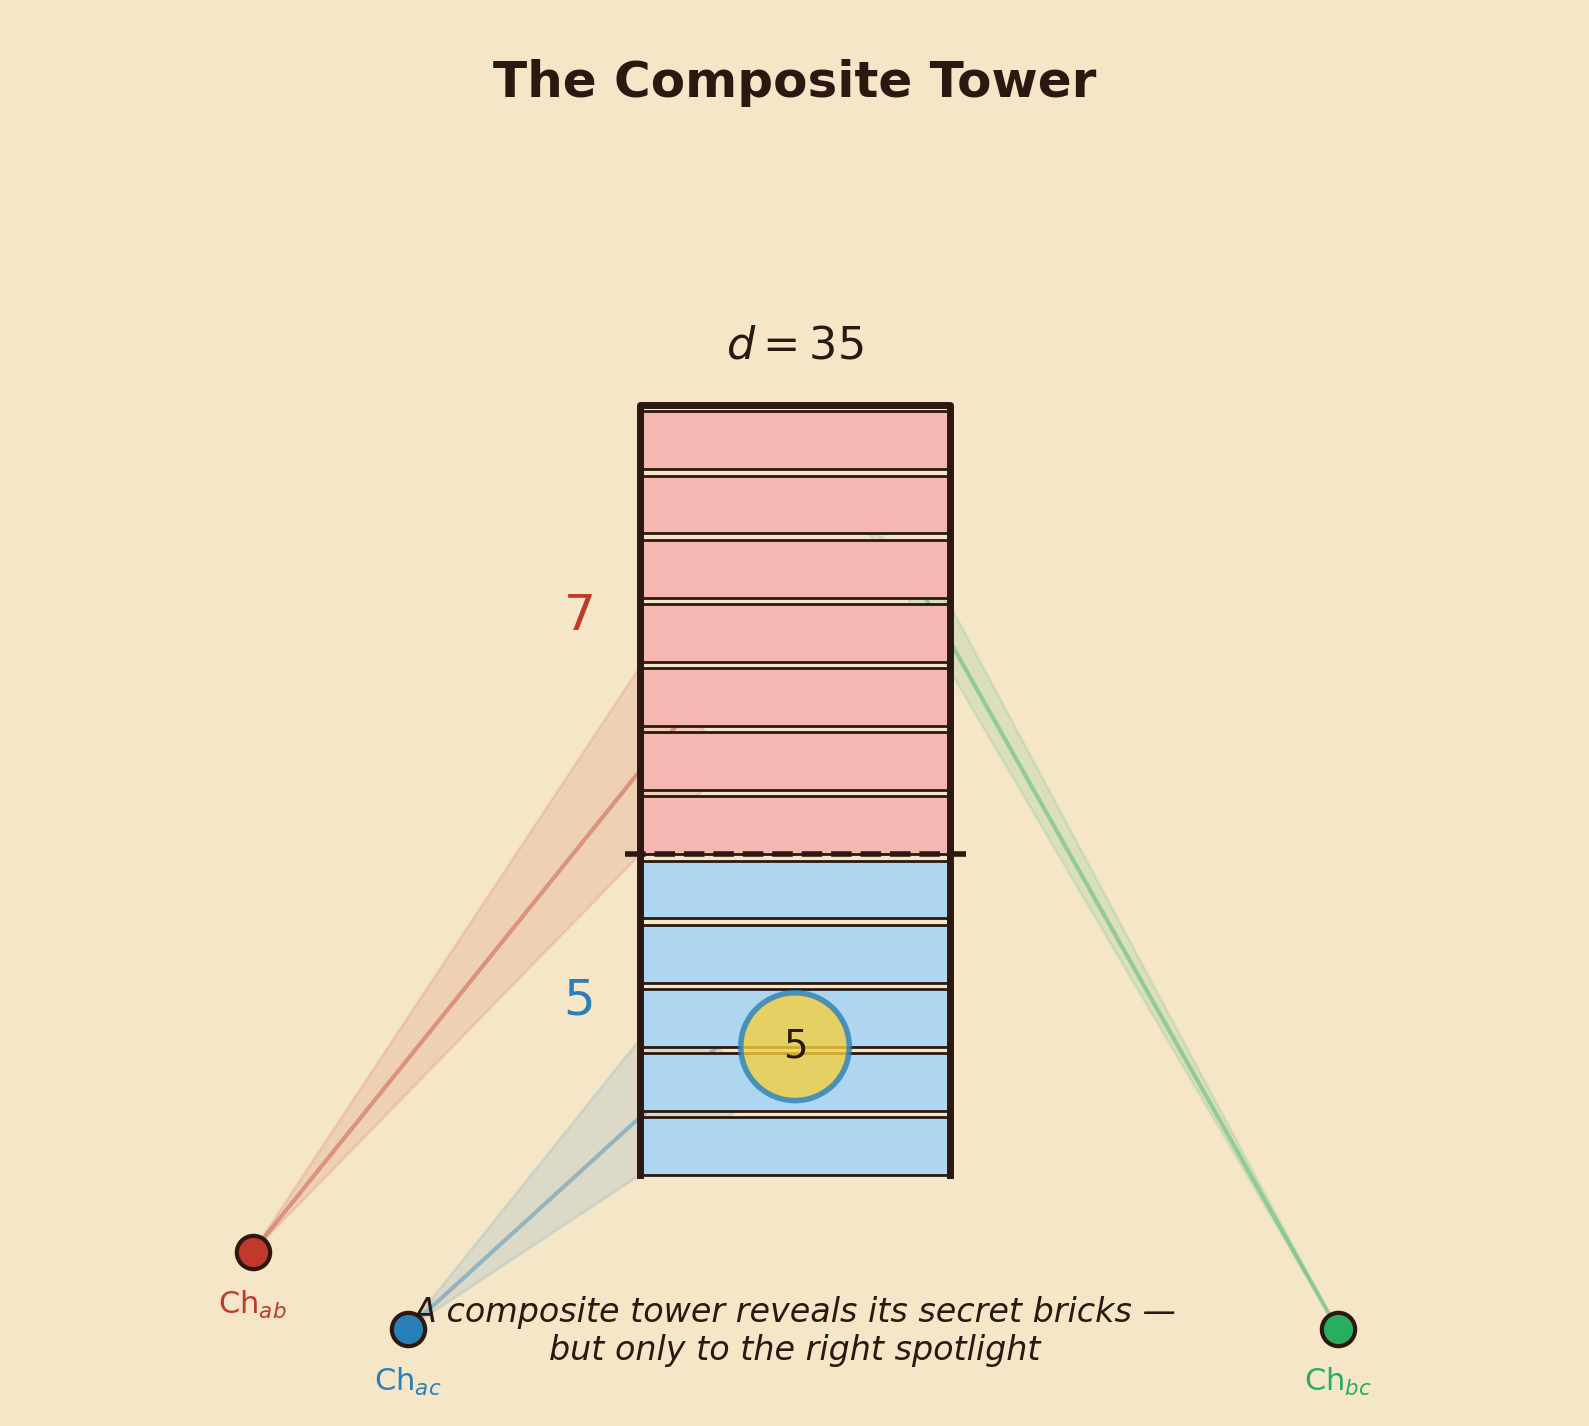
\includegraphics[width=0.82\textwidth]{../Chapter13/images/fig05_composite_tower.png}
\caption{A tall tower labeled $d = 35$ built from two colored brick layers: the bottom layer of $5$ blue bricks, the top layer of $7$ red bricks. Three spotlights from the base, labeled $\mathrm{Ch}_{ab}$,\ldots}
\end{figure}


\bigskip


\section{Even, Odd, and the Rule of Four}

Can you find four integers where exactly three of them are odd, their squares sum in the Pythagorean way $a^2 + b^2 + c^2 = d^2$, and the hypotenuse $d$ is even? Go ahead --- try.

You will fail, and the reason is a beautiful mod-$4$ obstruction. Every perfect square, when divided by $4$, leaves a remainder of $0$ or $1$. (Check: $0^2 \equiv 0$, $1^2 \equiv 1$, $2^2 \equiv 0$, $3^2 \equiv 1 \pmod{4}$.) If three of $a, b, c$ are odd, then $a^2 + b^2 + c^2 \equiv 1 + 1 + 1 = 3 \pmod{4}$. But $d^2$ can only be $0$ or $1$ mod $4$. Since $3$ is neither, no solution exists.

The mod-$4$ constraint is a gatekeeper. It forbids certain parity combinations outright, and it tightly constrains others. If $d$ is even, then $d^2 \equiv 0 \pmod{4}$, so $a^2 + b^2 + c^2 \equiv 0 \pmod{4}$. Since each square is $0$ or $1$ mod $4$, the only way to reach $0$ is for all three to be $0$ --- meaning $a$, $b$, and $c$ must \textit{all} be even. And if all three are even, we can divide through by $4$ and descend to a smaller quadruple. This "all-even descent" is itself a factoring tool: if $a = 2a'$, $b = 2b'$, $c = 2c'$, then $4(a'^2 + b'^2 + c'^2) = d^2$, so $2 \mid d$, say $d = 2d'$, and we obtain the reduced quadruple $(a', b', c', d')$.

The reader who recognizes the mod-$4$ obstruction from the theory of sums of three squares is seeing an old friend in new clothing. Legendre proved in 1798 that an integer $n$ is a sum of three squares if and only if $n$ is not of the form $4^k(8m + 7)$. The number $7$, for instance, cannot be written as $a^2 + b^2 + c^2$ for any integers $a, b, c$. The mod-$4$ obstruction we just uncovered is the same phantom, haunting a different corridor.

\begin{figure}[htbp]
\centering
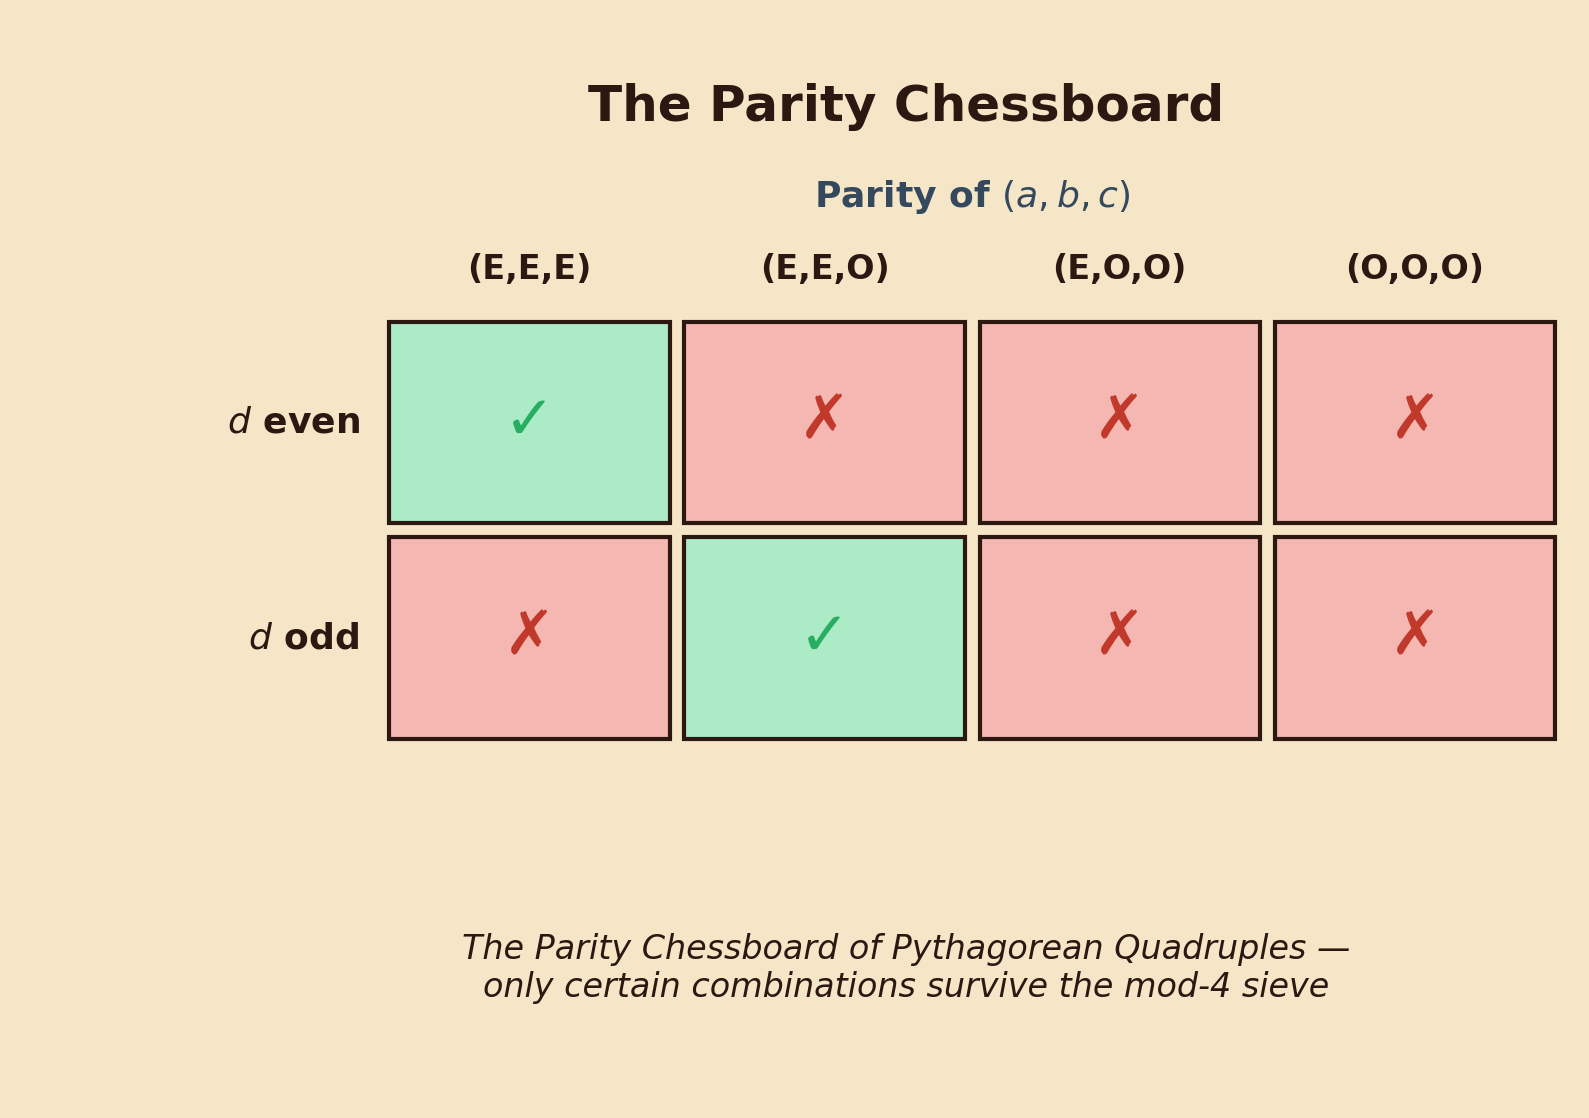
\includegraphics[width=0.82\textwidth]{../Chapter13/images/fig06_parity_chessboard.png}
\caption{A $4 \times 4$ grid. Columns are labeled with the parity patterns of $(a, b, c)$: $(E,E,E)$, $(E,E,O)$, $(E,O,O)$, $(O,O,O)$ --- where $E$ = even, $O$ = odd. Rows are labeled $d$ even, $d$ odd. Cells\ldots}
\end{figure}


\bigskip


\section{Many Witnesses, One Peak}

A number $d$ may sit atop not just one quadruple but many. Think of it as a mountain peak reachable by several different hiking trails. Each trail --- each representation --- sees a slightly different face of the mountain. By comparing the views from two trails, a hiker can triangulate a hidden feature invisible from either trail alone.

Suppose $(a_1, b_1, c_1, d)$ and $(a_2, b_2, c_2, d)$ are two quadruples sharing the same hypotenuse $d$. Then

\[
(a_1^2 + b_1^2) - (a_2^2 + b_2^2) = c_2^2 - c_1^2,
\]

because both sides equal $d^2 - c_1^2 - d^2 + c_2^2$. Now suppose $g \mid (d - c_1)$ and $g \mid (d - c_2)$. Subtracting: $g \mid (c_2 - c_1)$. If instead $g \mid (d - c_1)$ and $g \mid (d + c_2)$, then $g \mid (c_1 + c_2 + 2d - 2d)$... more carefully, from $d - c_1$ and $d + c_2$ we get $g \mid ((d + c_2) - (d - c_1)) = g \mid (c_1 + c_2)$. The cascade is \textit{transitive}: once the dominos start falling, every difference and sum of $c$-components topples.

With three representations --- three trails --- the cascade is devastating. If a prime $p$ divides $d - c_i$ for $i = 1, 2, 3$, then $p$ divides all six pairwise differences $c_i - c_j$. Three witnesses pointing at the same suspect; their testimony \textit{must} be consistent.

And the reverse cascade is equally potent: from $g \mid d$ and $g \mid (d - c)$, we immediately conclude $g \mid c$. Every factor of the hypotenuse that also divides a "gap" $d - c$ is a factor of the leg $c$ itself.

\begin{figure}[htbp]
\centering
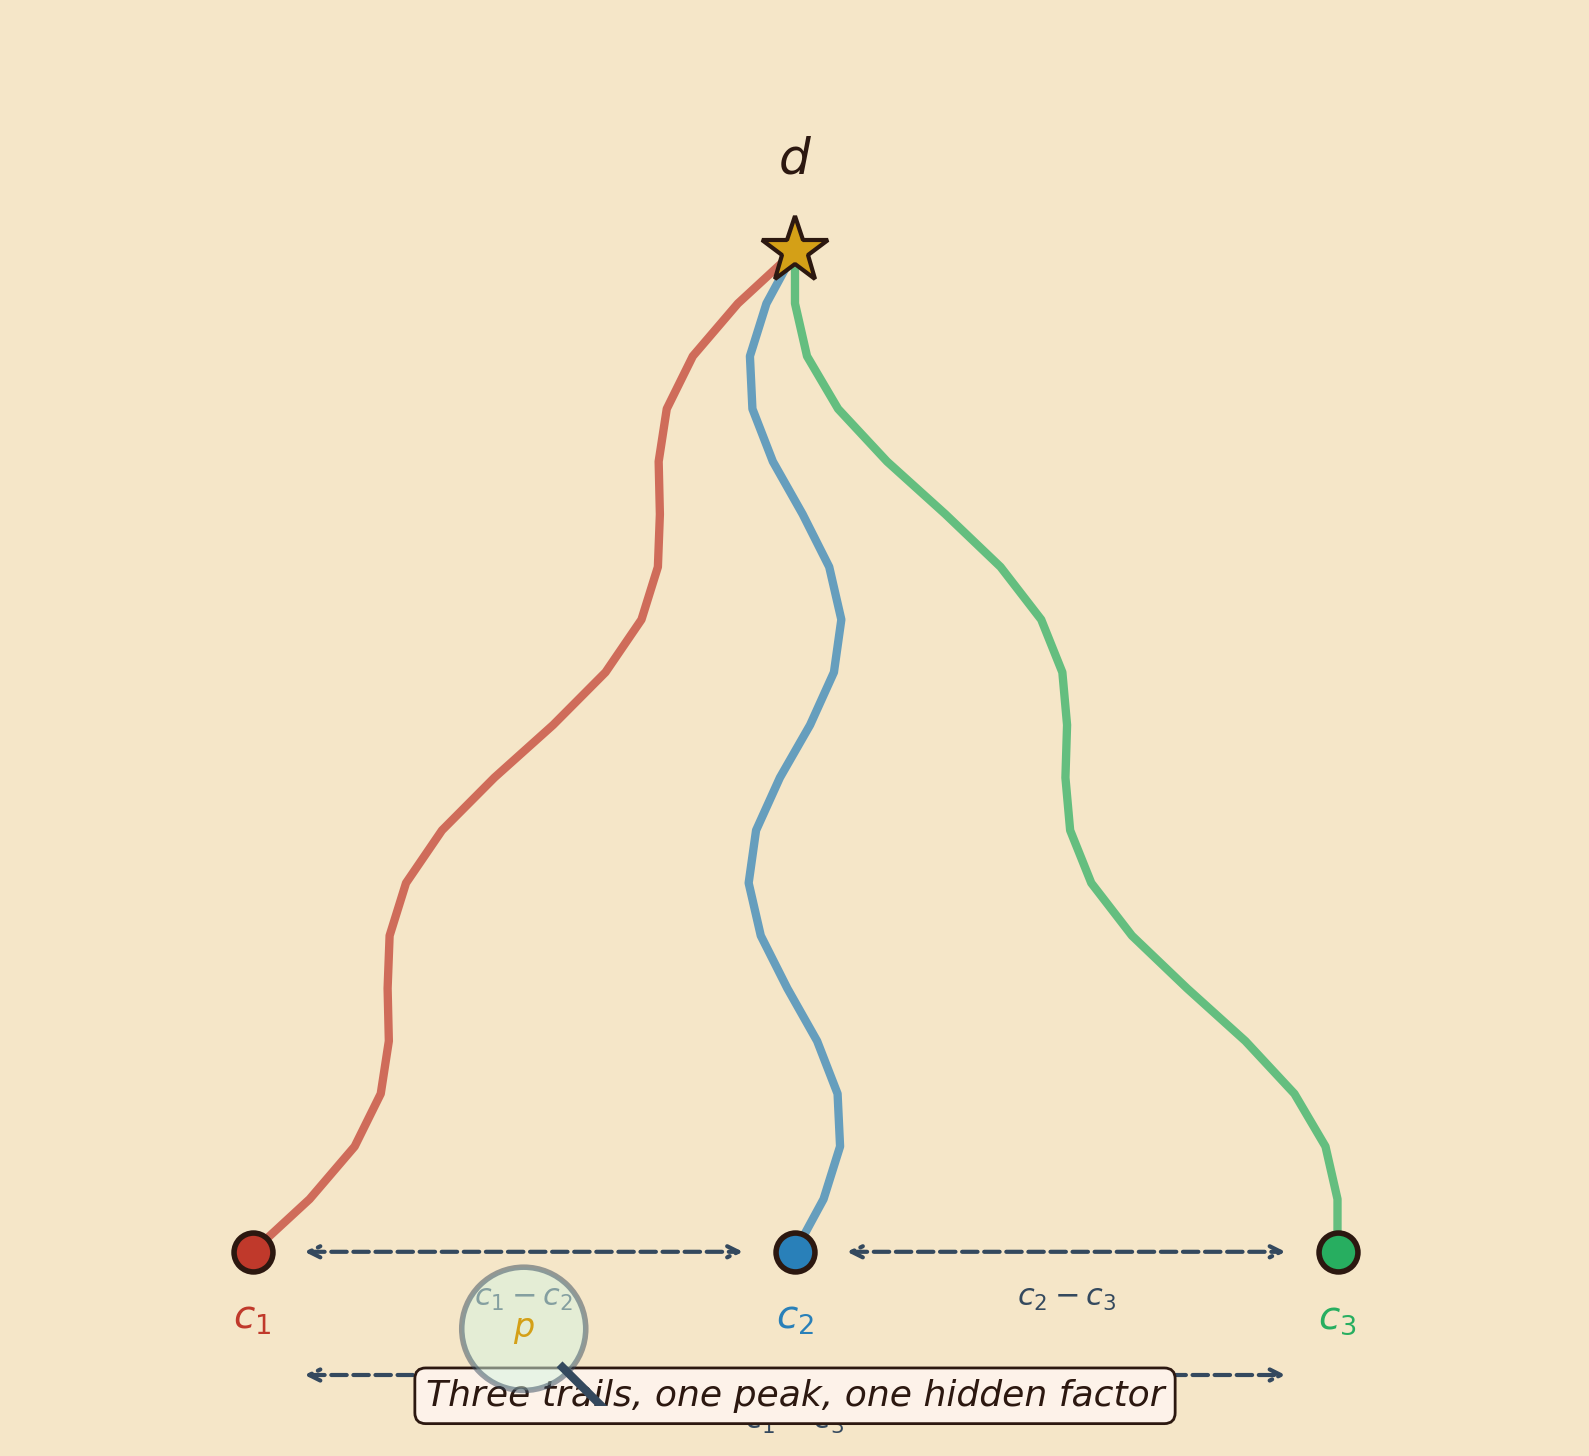
\includegraphics[width=0.82\textwidth]{../Chapter13/images/fig07_three_trails.png}
\caption{Three winding mountain trails converging on a single peak labeled $d$. Each trailhead at the base is labeled $c_1$, $c_2$, $c_3$ respectively. Dashed horizontal arrows connect pairs of trailheads,\ldots}
\end{figure}


\bigskip


\section{Brahmagupta's Ancient Trick}

In the seventh century, the Indian mathematician Brahmagupta discovered an identity so useful that it ought to be printed on the back of every business card in number theory.
\index{Brahmagupta}

Here is a puzzle to set the stage. Can you write $65$ as a sum of two squares? You might try: $65 = 64 + 1 = 8^2 + 1^2$. Good. Can you find another way? How about $65 = 49 + 16 = 7^2 + 4^2$? Now notice that $65 = 5 \times 13$, and $5 = 1^2 + 2^2$, and $13 = 2^2 + 3^2$. Is it a coincidence that the product of two sums-of-two-squares is itself a sum of two squares?

It is not. Brahmagupta proved the identity

\[
(a^2 + b^2)(c^2 + d^2) = (ac - bd)^2 + (ad + bc)^2 = (ac + bd)^2 + (ad - bc)^2.
\]

A product of sums-of-two-squares is itself a sum of two squares --- in \textit{two different ways}. For our example: $(1^2 + 2^2)(2^2 + 3^2) = (1 \cdot 2 - 2 \cdot 3)^2 + (1 \cdot 3 + 2 \cdot 2)^2 = (-4)^2 + 7^2 = 16 + 49 = 65$. And also $(1 \cdot 2 + 2 \cdot 3)^2 + (1 \cdot 3 - 2 \cdot 2)^2 = 8^2 + (-1)^2 = 64 + 1 = 65$. Both representations recovered from the factorization!

What does this have to do with Pythagorean channels? Everything. For a quadruple $(a, b, c, d)$, each channel $\mathrm{Ch}_{ab} = a^2 + b^2$ is a sum of two squares, and the channel's complementary form $d^2 - c^2 = (d-c)(d+c)$ is a product of two factors. The six small factors $(d \pm a)$, $(d \pm b)$, $(d \pm c)$ multiply to give the same result as the three channels:

\[
(d-a)(d+a) \cdot (d-b)(d+b) \cdot (d-c)(d+c) = \mathrm{Ch}_{bc} \cdot \mathrm{Ch}_{ac} \cdot \mathrm{Ch}_{ab}.
\]

The six small factors on the left are typically much easier to decompose than the three large channels on the right. This is where the real factoring power lives --- in the \textit{small} pieces, not the large ones. Brahmagupta, writing in his \textit{Br\={a}hmasphu{\d{t}}asiddh\={a}nta} in 628 CE, could not have dreamed that his identity would one day be the linchpin of a factoring cascade. Fibonacci rediscovered it in his \textit{Liber Quadratorum} in 1225. Euler generalized it further. The identity's quiet centrality to all of number theory has never faded.
\index{Fibonacci}
\index{Euler, Leonhard}

\begin{figure}[htbp]
\centering
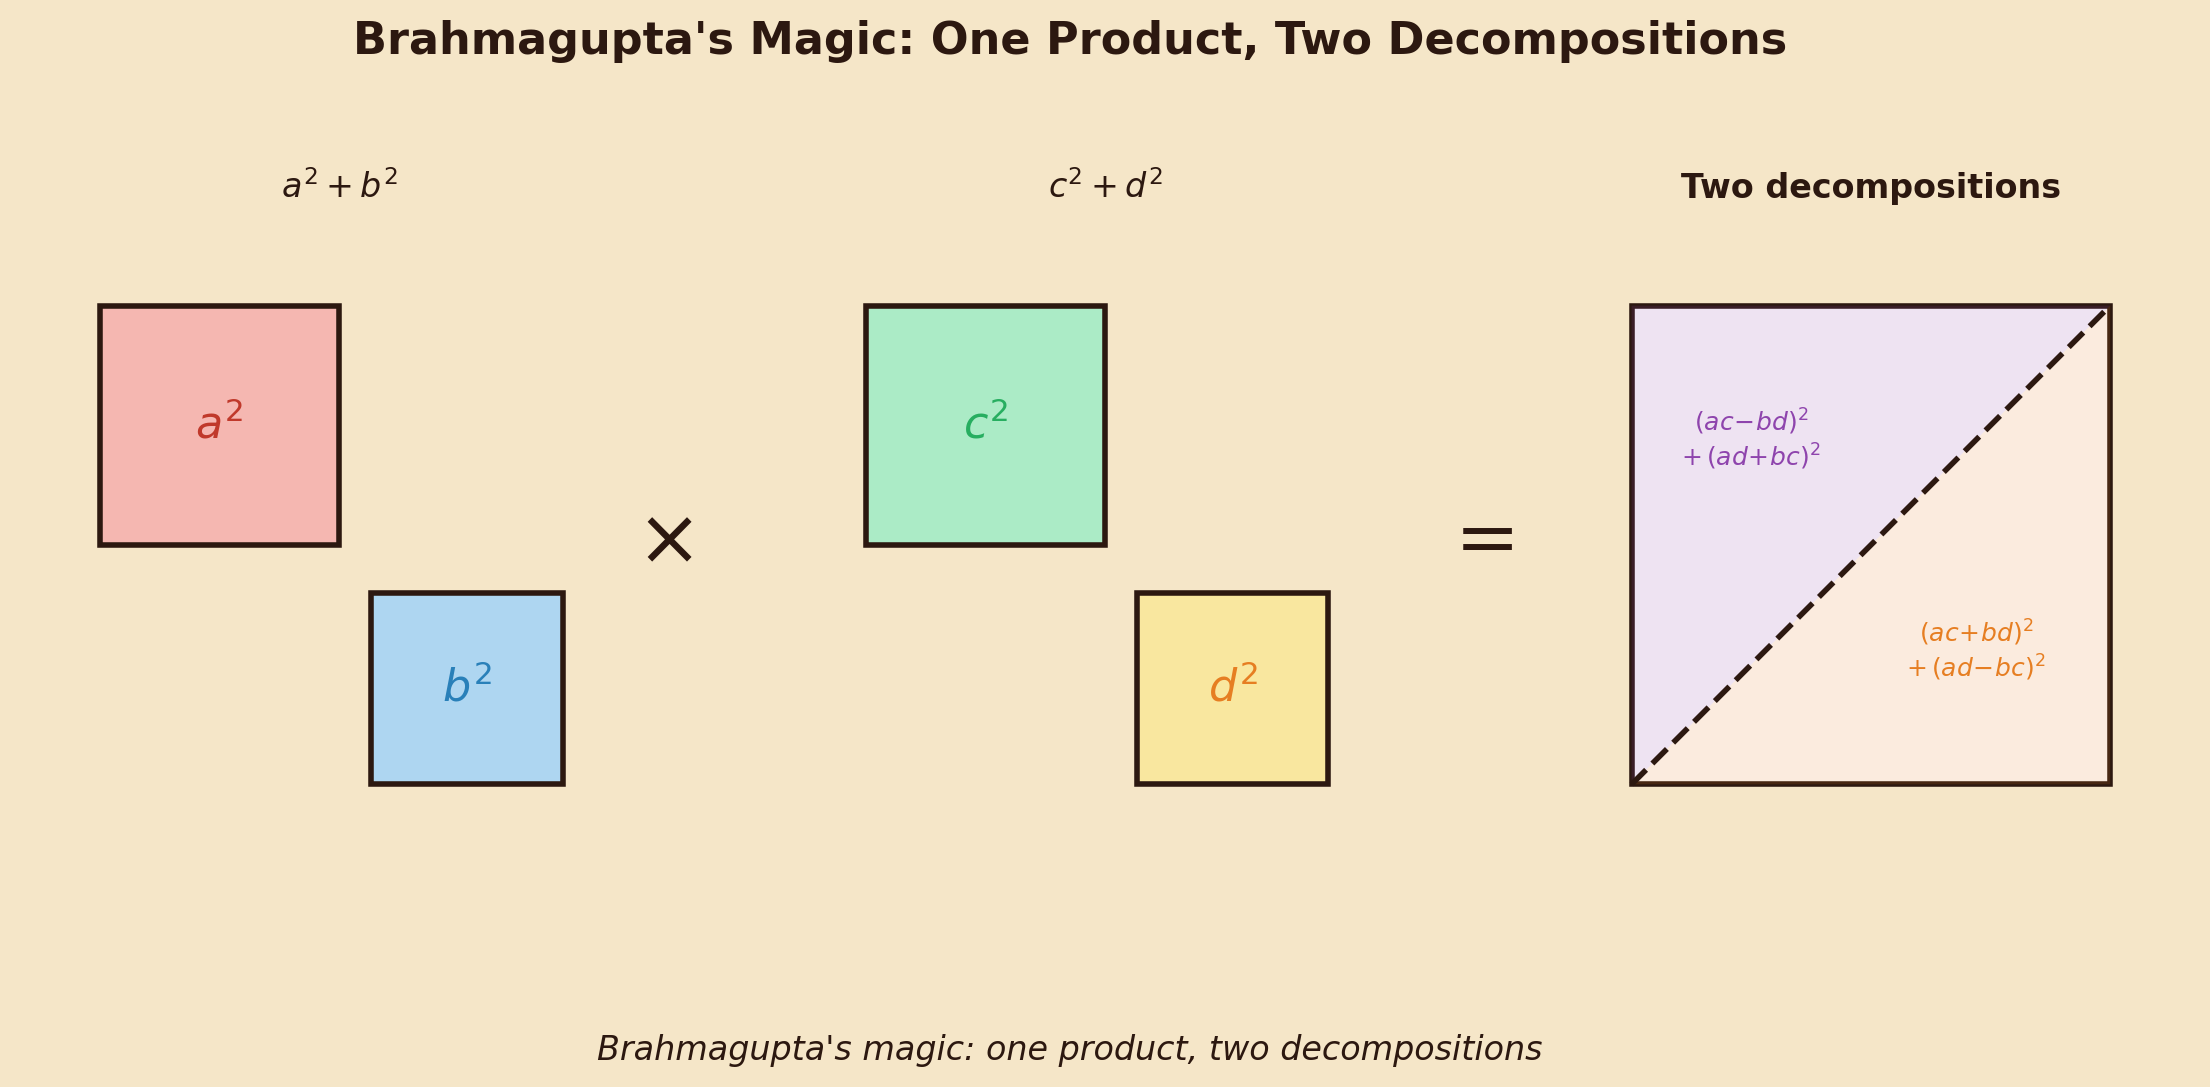
\includegraphics[width=0.82\textwidth]{../Chapter13/images/fig08_brahmagupta.png}
\caption{Two squares side by side, the first partitioned into sub-rectangles showing $a^2 + b^2$, the second showing $c^2 + d^2$. An arrow labeled "$\times$" points to a third, larger square partitioned\ldots}
\end{figure}


\bigskip


\section{The Factor Detective}

Imagine two crime scenes that share the same victim --- a composite number $d$. Each scene leaves behind different evidence (a different quadruple), but by cross-referencing the two sets of clues, a detective can identify the culprit: a nontrivial factor of $d$.

Here is the asymmetry that breaks the case. Suppose $p \mid d$ and $p \mid c_1$ in the first quadruple. Then $p^2 \mid \mathrm{Ch}_{ab}^{(1)} = d^2 - c_1^2$, because $p^2$ divides both $d^2$ and $c_1^2$. But in the second quadruple, suppose $p \nmid c_2$. Then $p^2 \nmid \mathrm{Ch}_{ab}^{(2)} = d^2 - c_2^2$, because $c_2^2$ is \textit{not} divisible by $p^2$ (even though $d^2$ is). The factor $p$ is \textit{visible} through one quadruple and \textit{invisible} through the other. This asymmetry is the detective's break in the case.

Return to our example: $d = 35$, first quadruple $(6, 10, 33, 35)$. We saw that $\mathrm{Ch}_{ac}^{(1)} = 1{,}125 = 5^3 \times 9$, where the factor $5$ screams because $5 \mid 35$ and $5 \mid 10$. Now consider a second quadruple, $(15, 10, 30, 35)$. Here $\mathrm{Ch}_{ac}^{(2)} = 15^2 + 30^2 = 225 + 900 = 1{,}125$ again --- not surprising, since $b = 10$ in both quadruples. But $\mathrm{Ch}_{ab}^{(2)} = 15^2 + 10^2 = 325 = 5^2 \times 13$, while $\mathrm{Ch}_{ab}^{(1)} = 6^2 + 10^2 = 136 = 8 \times 17$. The factor $5$ appears in the second quadruple's $\mathrm{Ch}_{ab}$ but \textit{not} in the first's. Cross-referencing reveals $5$ from every angle.

\begin{figure}[htbp]
\centering
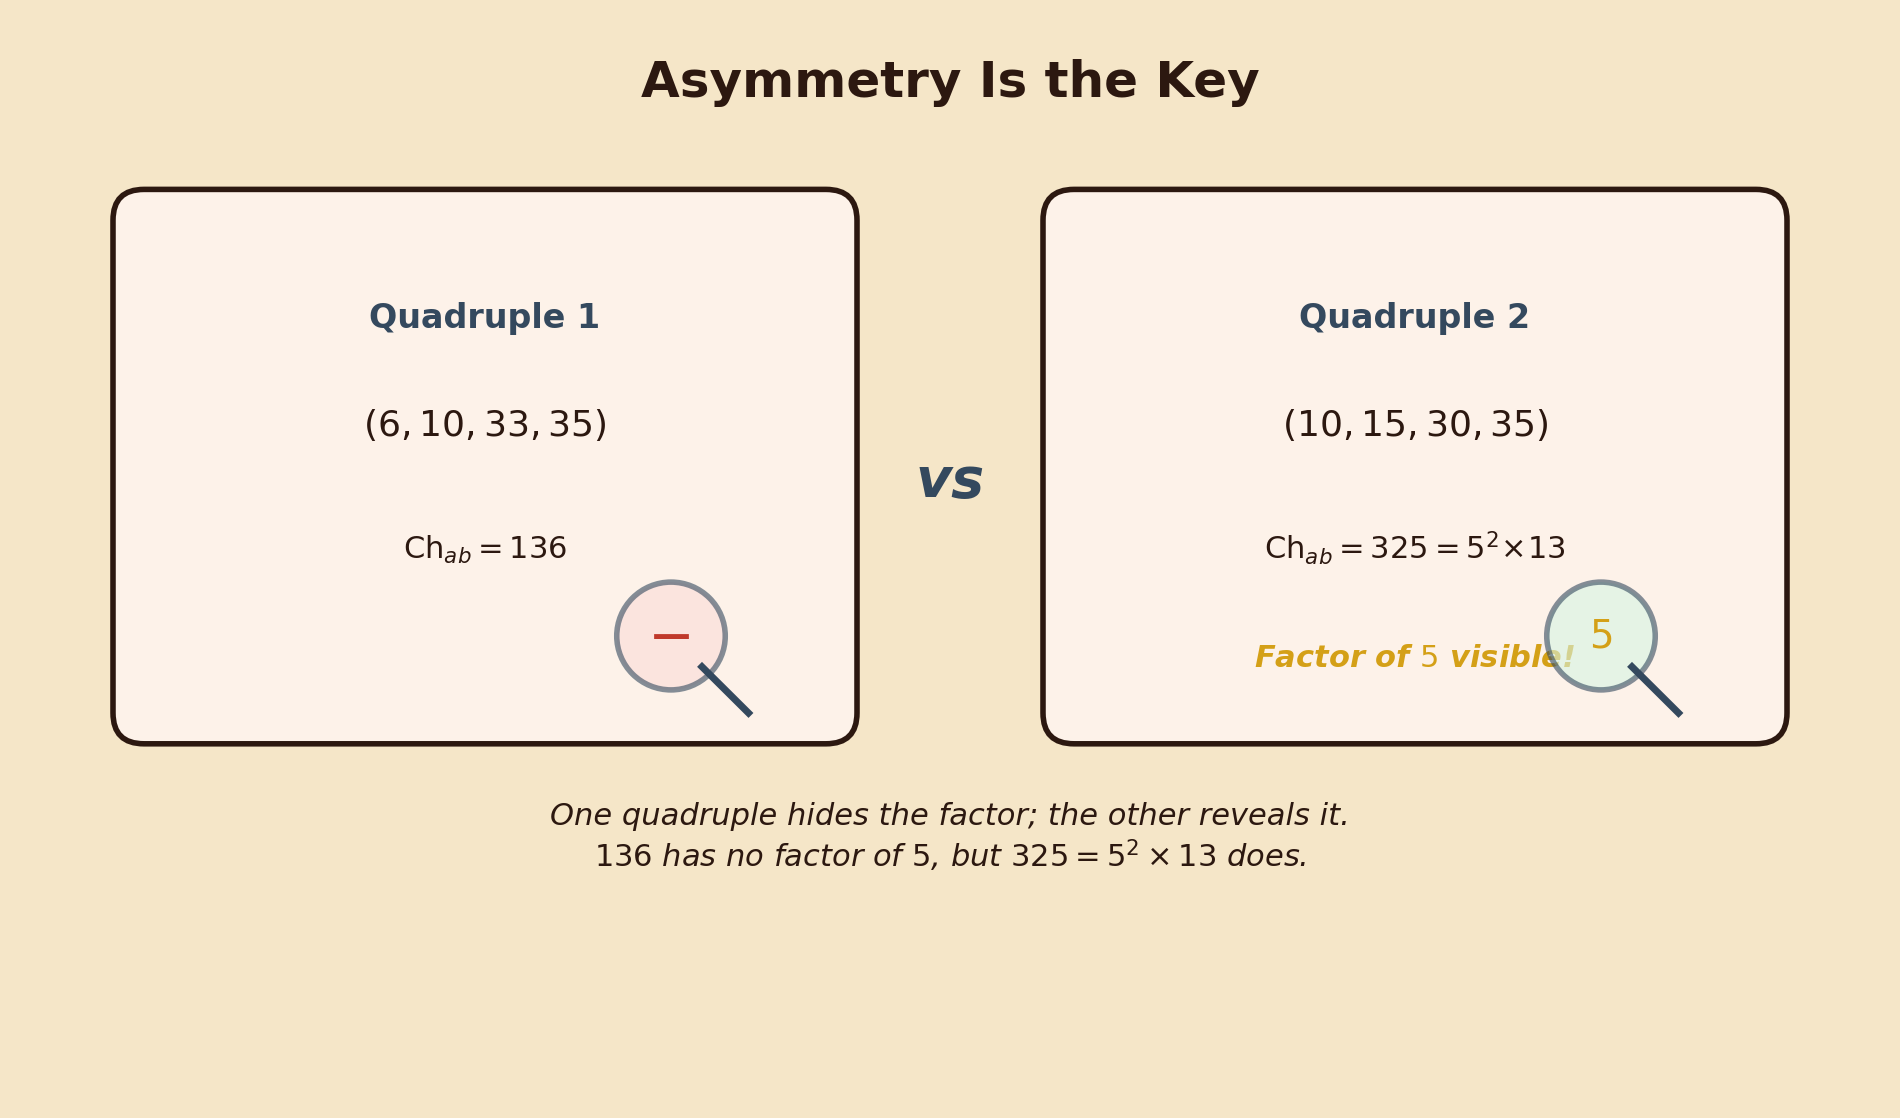
\includegraphics[width=0.82\textwidth]{../Chapter13/images/fig09_asymmetry.png}
\caption{Two magnifying glasses hovering over two index cards, each showing a different quadruple for $d = 35$. One glass reveals a glowing "$5$" in its channel value; the other shows a blank where the $5$\ldots}
\end{figure}


\bigskip


\section{Infinite Descent Among the Quadruples}

Pierre de Fermat's favorite trick was \textit{infinite descent}: prove that if a solution exists, a smaller one must also exist, and then a still smaller one, and so on --- until you reach an impossibility. What if we turn descent into a \textit{tool} rather than a contradiction?
\index{Fermat, Pierre de}
\index{descent!infinite}

If a prime $p$ divides all three spatial components $a$, $b$, $c$ in a quadruple, write $a = pa'$, $b = pb'$, $c = pc'$. Then

\[
p^2(a'^2 + b'^2 + c'^2) = d^2,
\]

so $p^2 \mid d^2$, and since $p$ is prime, $p \mid d$. Write $d = pd'$. The quadruple $(a, b, c, d)$ contains a \textit{smaller} quadruple $(a', b', c', d')$ inside it, scaled down by $p$. If $(a', b', c')$ are again all divisible by $p$, descend once more. The components are shrinking --- they are positive integers, after all --- so the process must terminate. When it does, it has peeled off the full power of $p$ dividing $d$.

Descent \textit{is} division, made geometric. Each step zooms in on a smaller copy of the same structure, like a fractal viewed at finer and finer resolution. The outermost quadruple lives on a sphere of radius $d$; the next lives on a sphere of radius $d/p$; the next on $d/p^2$. Fermat used descent to prove impossibilities. We use it to extract factors.

\begin{figure}[htbp]
\centering
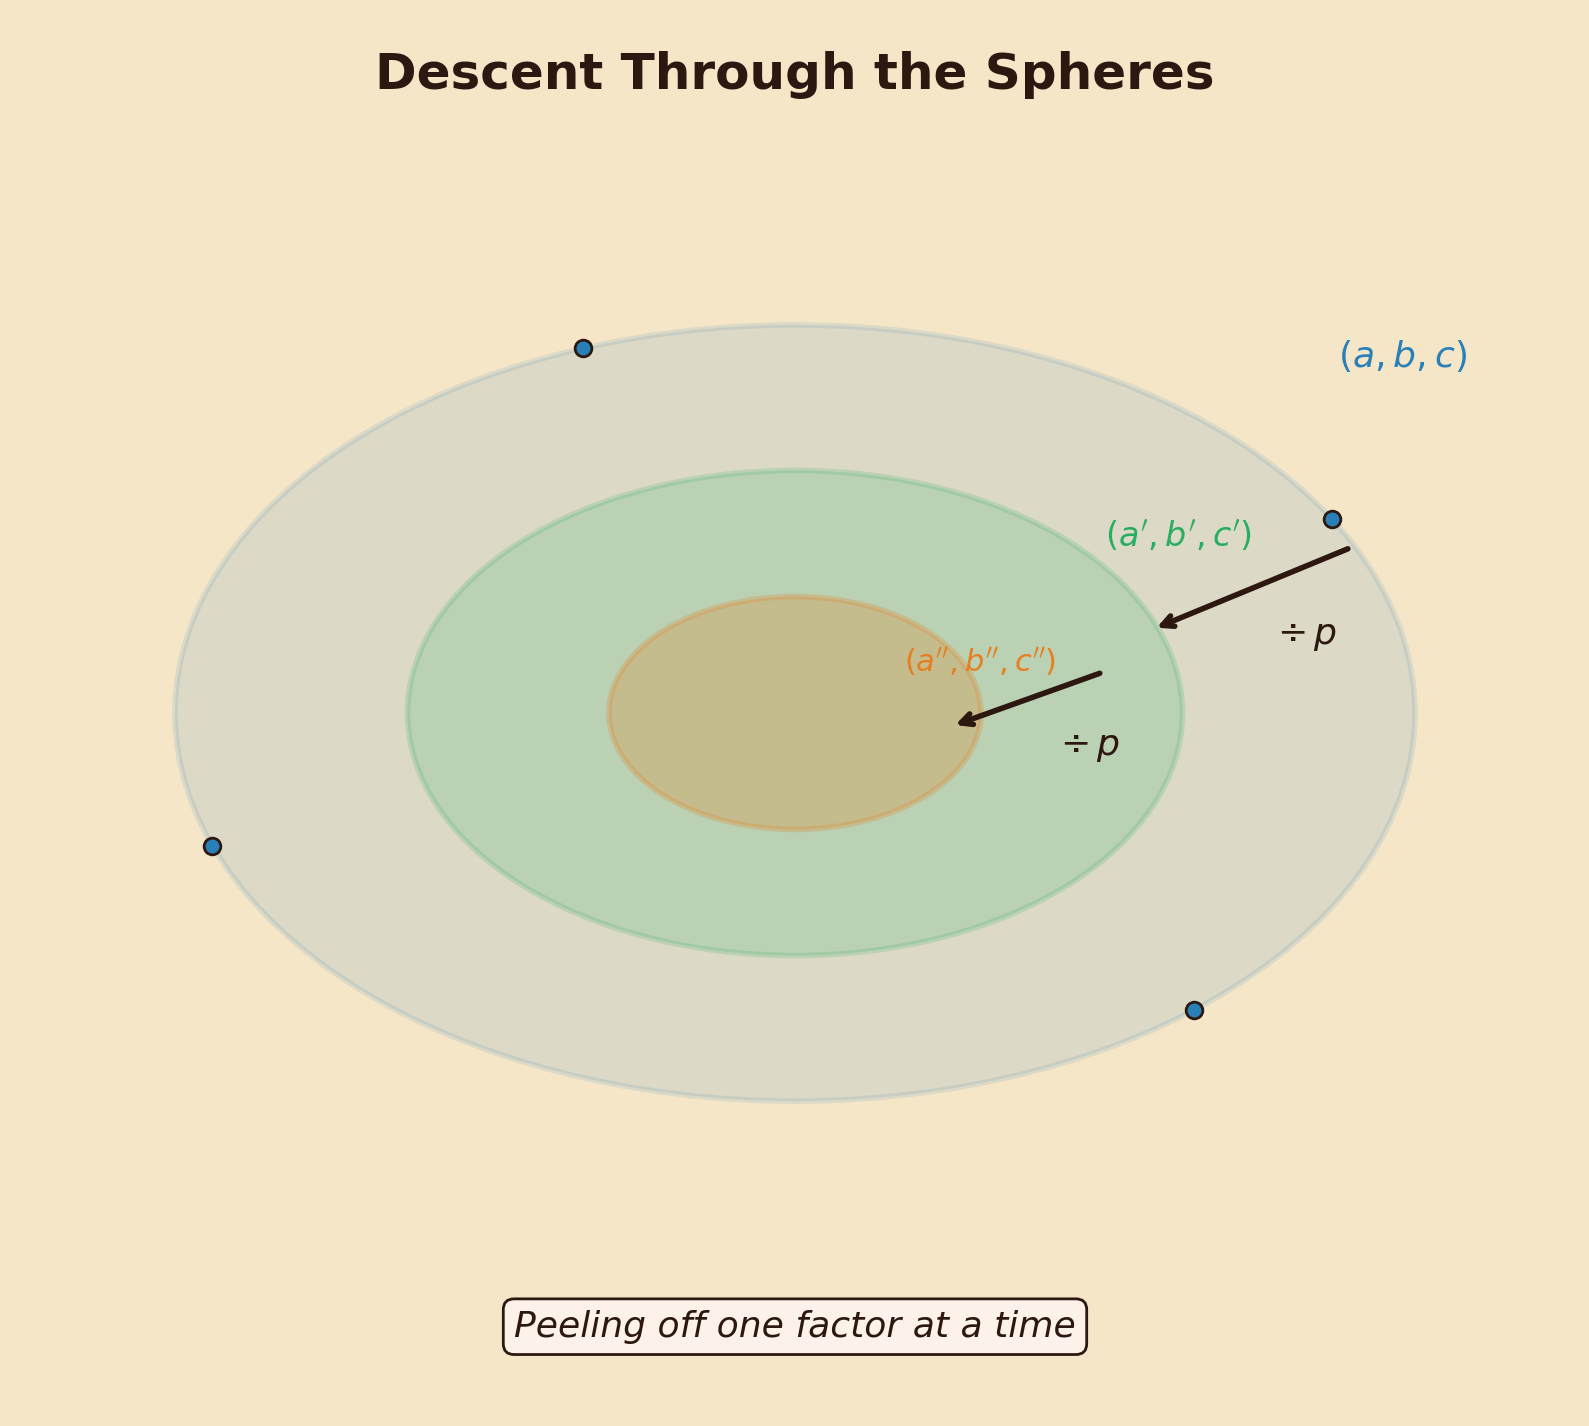
\includegraphics[width=0.82\textwidth]{../Chapter13/images/fig10_descent_spheres.png}
\caption{A nested sequence of three concentric translucent spheres, each smaller by a factor of $p$. The outermost sphere has lattice points $(a, b, c)$ marked on its surface. The next inner sphere shows\ldots}
\end{figure}


\bigskip


\section{The Balanced Quadruple That Doesn't Exist}

What if all three legs of a Pythagorean quadruple were equal? Then we would need

\[
3a^2 = d^2,
\]

which gives $d/a = \sqrt{3}$. But $d$ and $a$ are integers --- their ratio is rational. And $\sqrt{3}$ is not. Contradiction. There is no nonzero integer solution.

This tiny proof --- three lines, barely a paragraph --- conceals a deep principle. The irrationality of $\sqrt{3}$ follows from the fact that $3$ is prime, which prevents $3a^2 = d^2$ from having a solution (since $3$ would have to divide $d$, say $d = 3d'$, giving $a^2 = 3d'^2$, which forces $3 \mid a$, say $a = 3a'$, giving $3a'^2 = d'^2$ --- infinite descent again, with no base case).

But if perfect balance is impossible, what about \textit{near} balance? Set $a = b$. The equation becomes $2a^2 + c^2 = d^2$, i.e., $(d - c)(d + c) = 2a^2$. This is solvable --- and it connects to one of the oldest equations in mathematics. Set $c = 1$:

\[
d^2 - 2a^2 = 1.
\]

This is the \textbf{Pell equation}! Its solutions march onward forever: $(a, d) = (2, 3), (12, 17), (70, 99), (408, 577), \ldots$, each pair generating the nearly-balanced quadruple $(a, a, 1, d)$. The ratios $d/a = 3/2, 17/12, 99/70, 577/408, \ldots$ converge to $\sqrt{2}$ --- closer and closer, but never arriving. The balanced quadruple is the limit of an infinite staircase, forever approached, never reached.
\index{Pell equation}

A historical footnote that delights and exasperates in equal measure: the equation $x^2 - Ny^2 = 1$ is called "Pell's equation," but John Pell had almost nothing to do with it. The real credit belongs to Lord Brouncker, who solved it in 1657 at Fermat's challenge, and to the Indian mathematicians Brahmagupta (him again!) and Bh\={a}skara II, who had studied it centuries earlier. Euler attributed it to Pell by mistake, and the name stuck. Mathematics is littered with such misattributions --- Stigler's Law of Eponymy states that no scientific discovery is named after its actual discoverer, and Stigler's Law is itself named after someone who didn't discover it.

\begin{figure}[htbp]
\centering
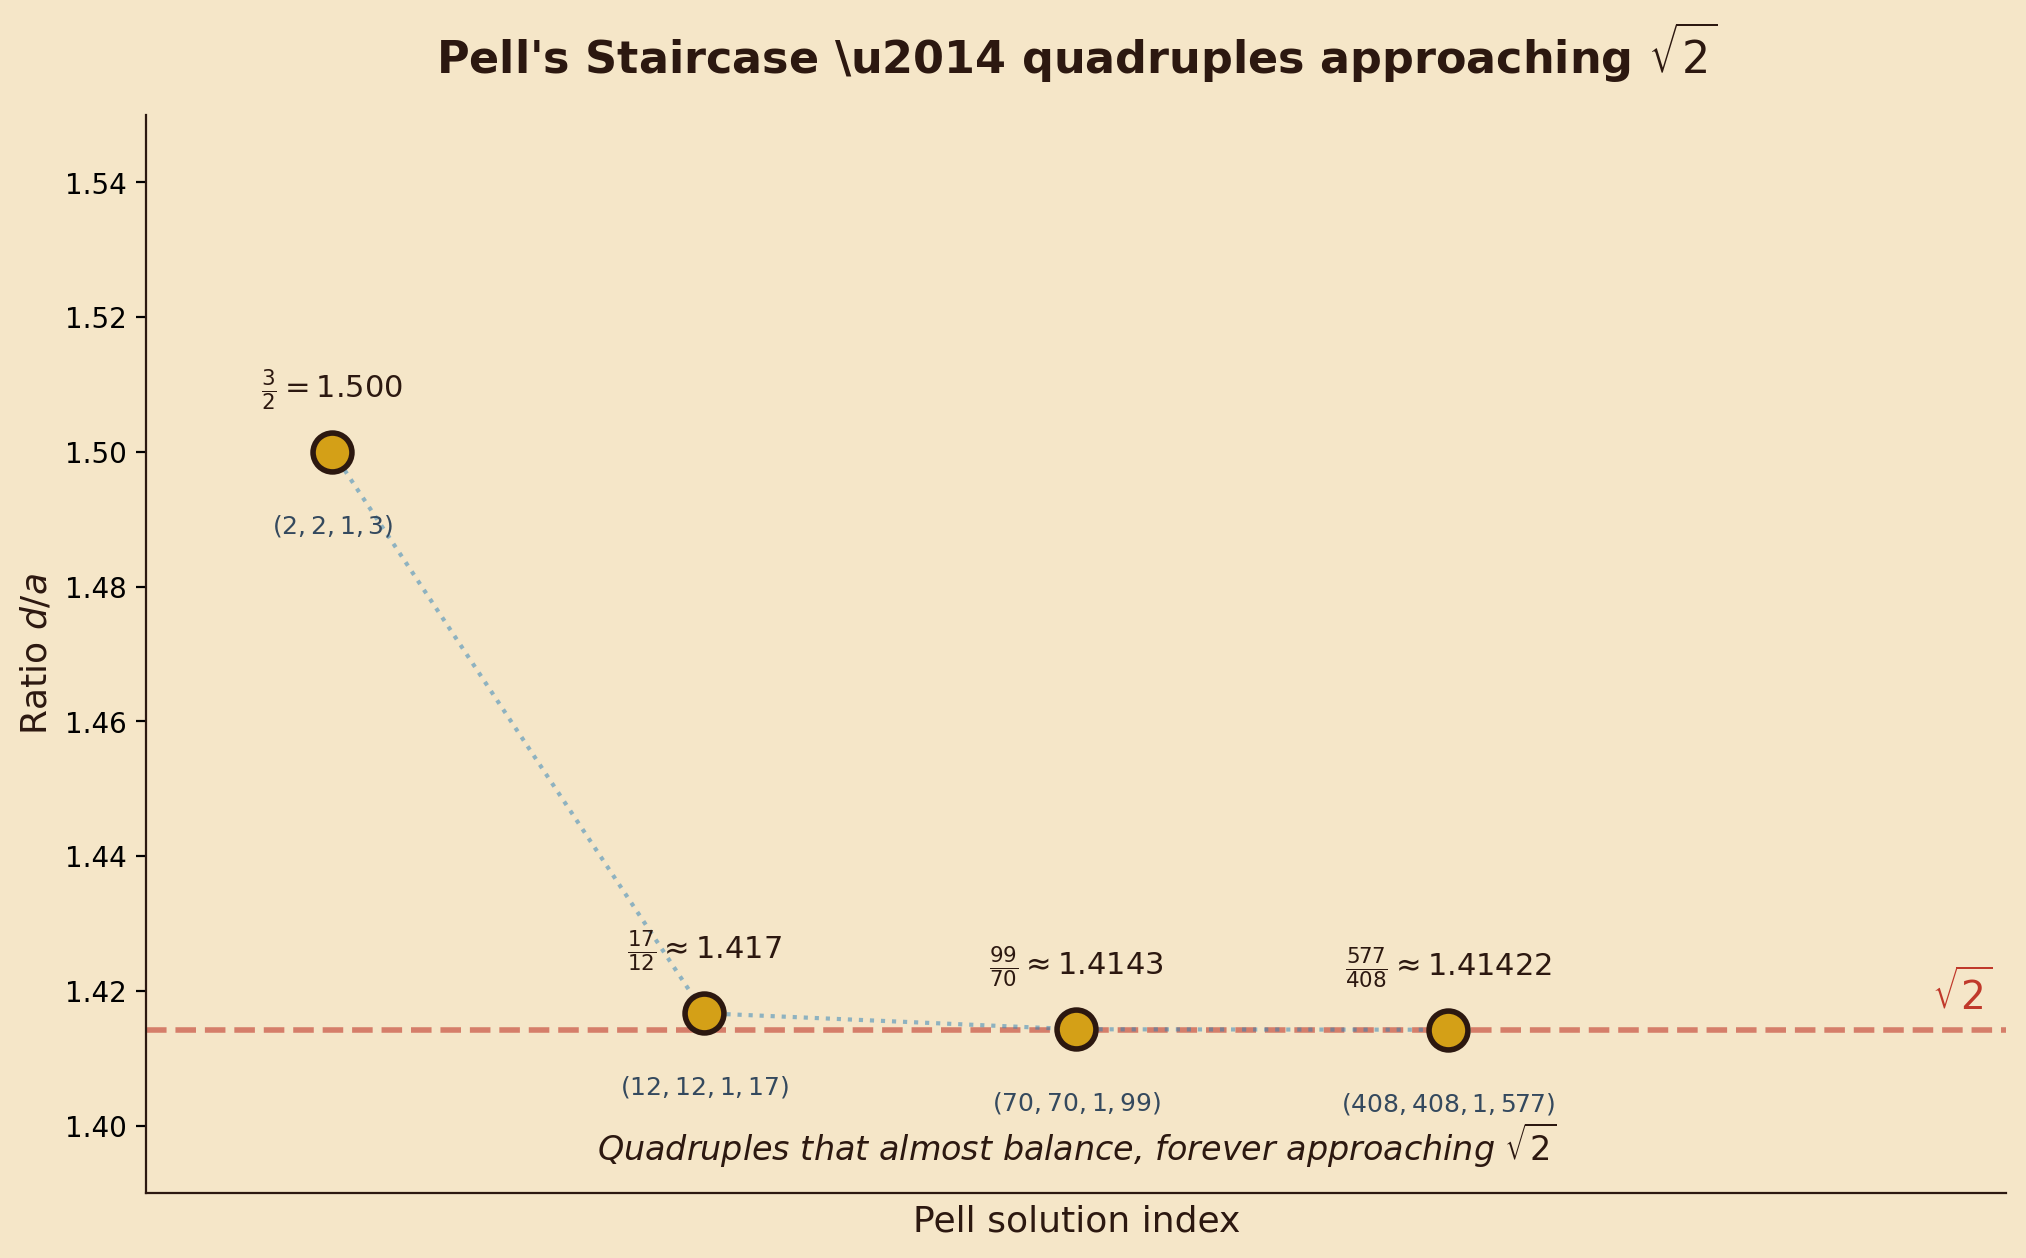
\includegraphics[width=0.82\textwidth]{../Chapter13/images/fig11_pell_staircase.png}
\caption{A number line from $1.0$ to $1.5$ showing the ratios $d/a$ for successive Pell solutions: $3/2 = 1.500$, $17/12 = 1.417$, $99/70 = 1.414\overline{285}$, $577/408 = 1.41421\overline{568}$. A dashed\ldots}
\end{figure}


\bigskip


\section{Higher Dimensions, Higher Channels}

Everything we have done works in three spatial dimensions. What happens in four? Five? A hundred?

For $n$ spatial components satisfying $a_1^2 + a_2^2 + \cdots + a_n^2 = d^2$, there are $\binom{n}{2}$ pairwise channels $a_i^2 + a_j^2$. Each component $a_i^2$ appears in exactly $n - 1$ of them, so the channel sum is

\[
\sum_{1 \le i < j \le n} (a_i^2 + a_j^2) = (n - 1)(a_1^2 + a_2^2 + \cdots + a_n^2) = (n - 1) \cdot d^2.
\]

For $n = 3$ (the quadruple), we recover $\binom{3}{2} = 3$ channels summing to $2d^2$. For $n = 4$ (the quintuplet), $6$ channels sum to $3d^2$. For $n = 5$ (the sextuplet), $10$ channels sum to $4d^2$. The pattern is pure double-counting --- the simplest idea in combinatorics hiding the deepest consequences. And all the cross-channel GCD results from earlier generalize: if $g$ divides all $\binom{n}{2}$ channels, then $g$ divides $2a_i^2$ for every $i$, by the same linear-combination trick.

\begin{figure}[htbp]
\centering
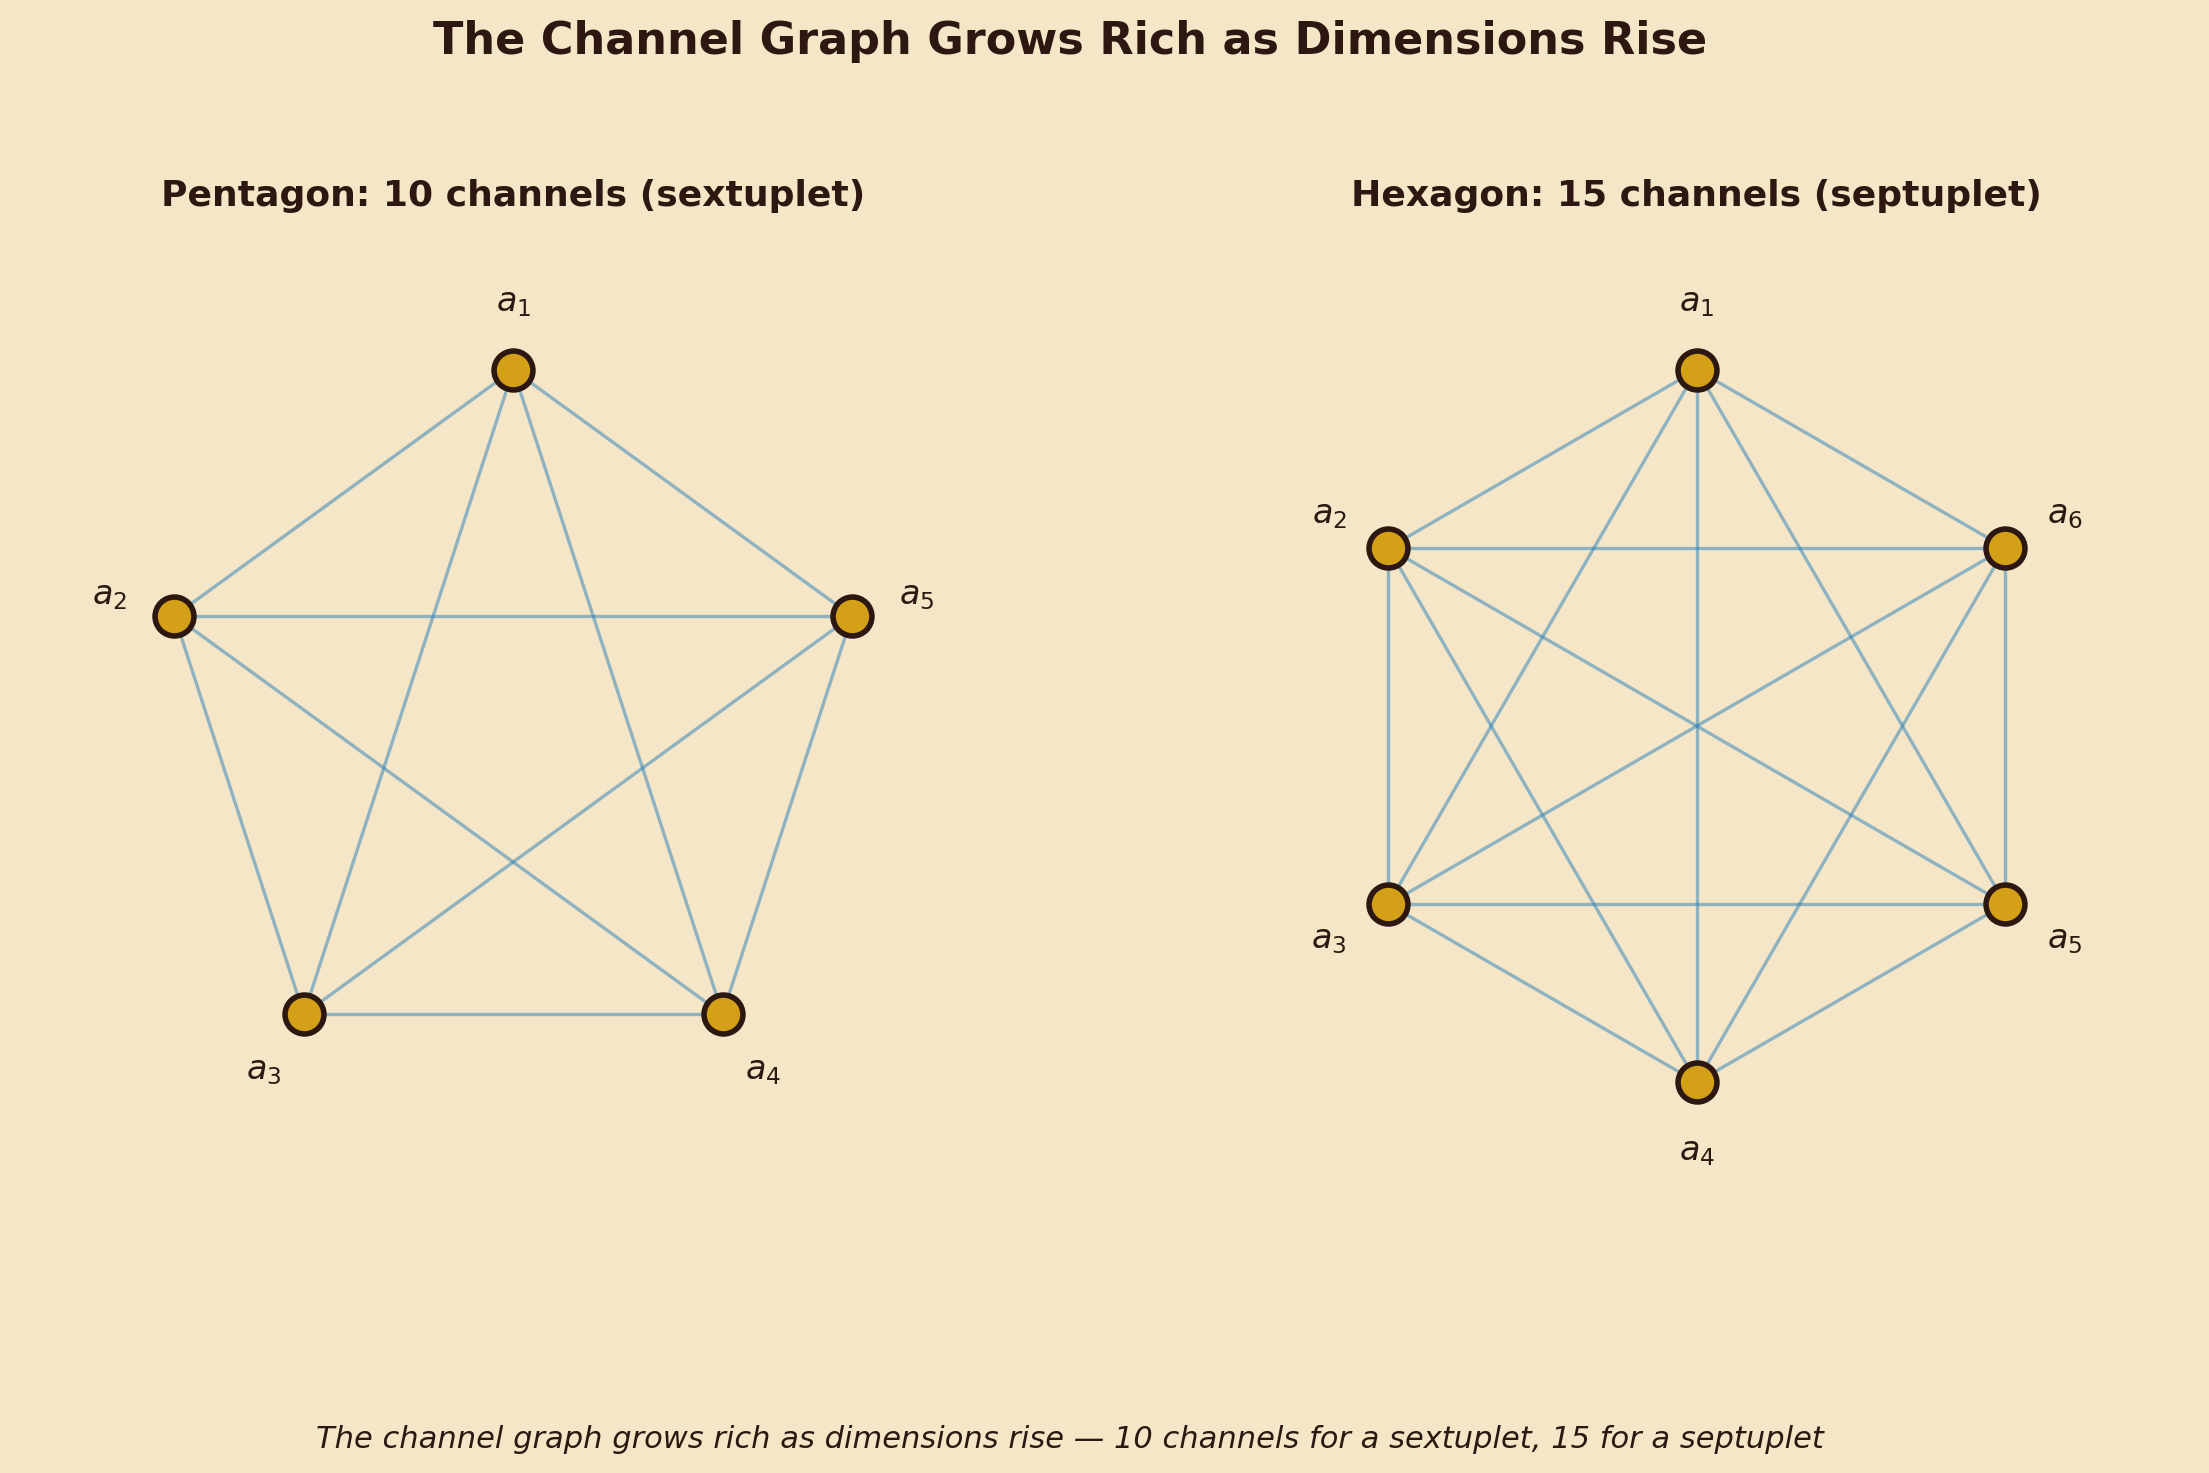
\includegraphics[width=0.82\textwidth]{../Chapter13/images/fig12_channel_graphs.png}
\caption{A pentagon with vertices labeled $a_1, a_2, a_3, a_4, a_5$ and all $10$ edges and diagonals drawn, each labeled with a channel value $a_i^2 + a_j^2$. Beside it, a hexagon with vertices labeled\ldots}
\end{figure}


\bigskip


\section{Fingerprints and Sieves}

Every composite number leaves a fingerprint --- a pattern of residues modulo its prime factors. The channels of a Pythagorean quadruple are like an ink pad: press the hypotenuse against them, and its prime fingerprint transfers perfectly.

If $p \mid d$, then $p^2 \mid d^2 = a^2 + b^2 + c^2$. Every quadruple sharing the same hypotenuse $d$ must satisfy this constraint: $(a^2 + b^2 + c^2) \equiv 0 \pmod{p^2}$. Two different quadruples for the same $d$ leave the \textit{same} fingerprint, because $(a_1^2 + b_1^2 + c_1^2) - (a_2^2 + b_2^2 + c_2^2) = d^2 - d^2 = 0$.

There is also a channel-level fingerprint. If $p \mid a$, then $p \mid (a^2 + b^2)$ if and only if $p \mid b$. A prime that divides one leg of a channel can \textit{see through} to the other leg. And this leads to a lovely generation trick: if $a^2 + b^2 = (2k + m) \cdot m$ for some integers $k$ and $m$, then

\[
a^2 + b^2 + k^2 = k^2 + 2km + m^2 = (k + m)^2.
\]

Every factorization of a sum of two squares \textit{is} a Pythagorean quadruple in disguise, with $c = k$ and $d = k + m$. This simple observation --- almost too simple to dignify as a theorem --- is the engine that generates quadruples from factorizations. And since the small factor $d - c = m$ is always a positive divisor of $\mathrm{Ch}_{ab}$ less than $d$, it is a lever: smaller than the hypotenuse itself, yet sufficient to pry it apart.

\begin{figure}[htbp]
\centering
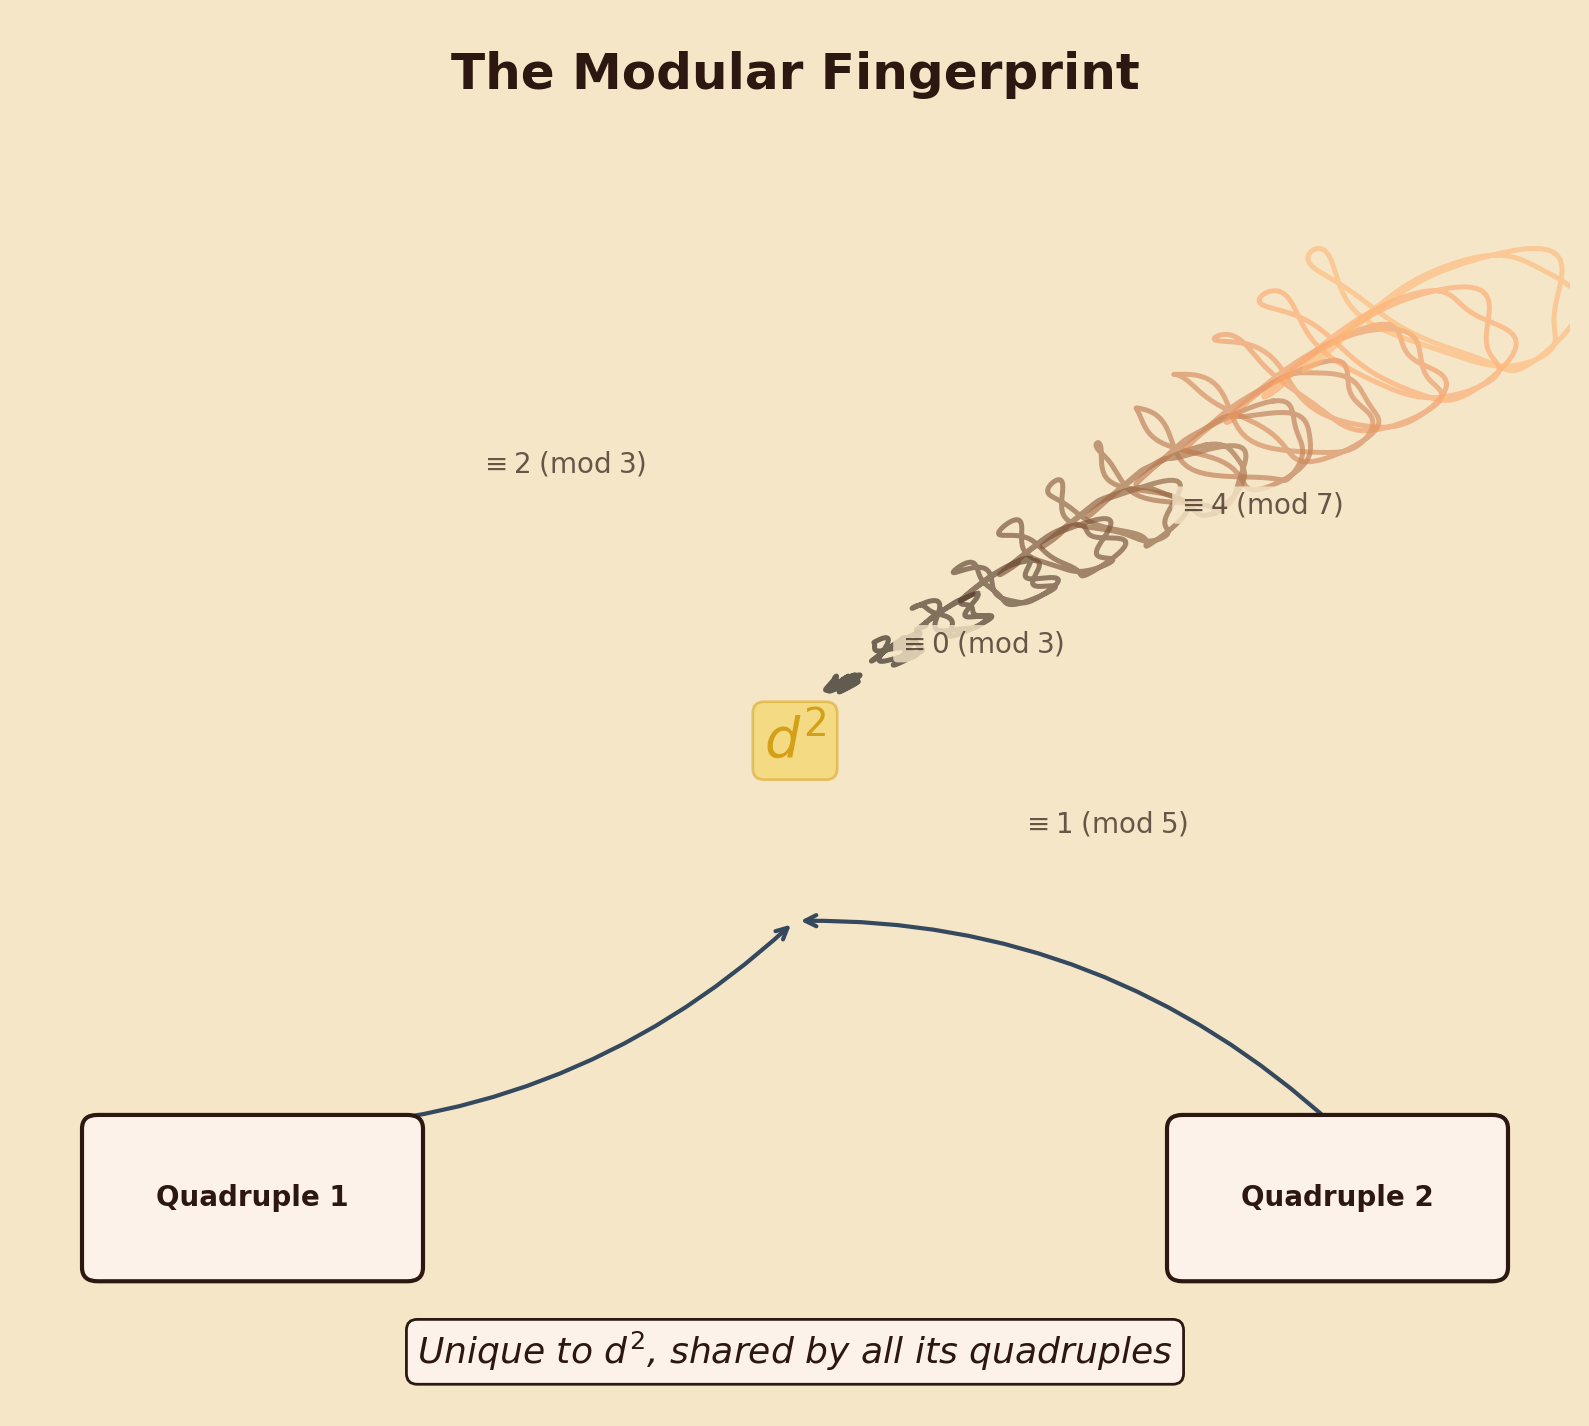
\includegraphics[width=0.82\textwidth]{../Chapter13/images/fig13_modular_fingerprint.png}
\caption{A large thumbprint pattern where the ridges are formed by concentric ellipses. Each elliptical ridge is labeled with a residue $a^2 + b^2 + c^2 \pmod{p^2}$ for a small prime $p$ (e.g., $p = 3$ and\ldots}
\end{figure}


\bigskip


\section{Putting It All Together}

Let us watch the entire machinery in action.

**Example 1: $d = 35 = 5 \times 7$.** Take the quadruple $(6, 10, 33, 35)$. Compute the three factored channels:

\[
d - a = 29, \quad d + a = 41, \quad \mathrm{Ch}_{bc} = 29 \times 41 = 1{,}189.
\]

\[
d - b = 25, \quad d + b = 45, \quad \mathrm{Ch}_{ac} = 25 \times 45 = 1{,}125.
\]

\[
d - c = 2, \quad d + c = 68, \quad \mathrm{Ch}_{ab} = 2 \times 68 = 136.
\]

Now: $\gcd(d - b, d) = \gcd(25, 35) = 5$. Done. One GCD, one factor. The channel $\mathrm{Ch}_{ac}$ betrayed the prime $5$ because $5$ divided both $d$ and $b$, making $d - b = 25$ a multiple of $5$.

**Example 2: $d = 15 = 3 \times 5$.** Take $(2, 10, 11, 15)$. Then $d - b = 5$, and $\gcd(5, 15) = 5$. Instant factorization.

**Example 3: $d = 21 = 3 \times 7$.** Take $(6, 9, 18, 21)$. Then $d - c = 3$, and $\gcd(3, 21) = 3$. The factor $3$ falls out before you have time to sharpen your pencil.

The "algorithm," if we dare call something so ancient by so modern a name, is this:

\begin{enumerate}
\item Start with a composite $d$.
\item Find one or more quadruples $(a, b, c, d)$ with $a^2 + b^2 + c^2 = d^2$.
\item Compute the six small factors: $d - a$, $d + a$, $d - b$, $d + b$, $d - c$, $d + c$.
\item Take $\gcd(d - x, d)$ for each component $x \in \{a, b, c\}$. Any nontrivial GCD reveals a factor.
\item If all GCDs are trivial, cross-reference with a second quadruple and apply the cascade.
\end{enumerate}
The method is not guaranteed to succeed with a single quadruple --- it is possible, though rare, for all six small factors to be coprime to $d$. But with multiple representations, the probability of detection compounds. And the cascade ensures that even a single detected prime propagates through the entire structure, exposing all the factors of $d$ in a chain reaction of divisibility.

\begin{figure}[htbp]
\centering
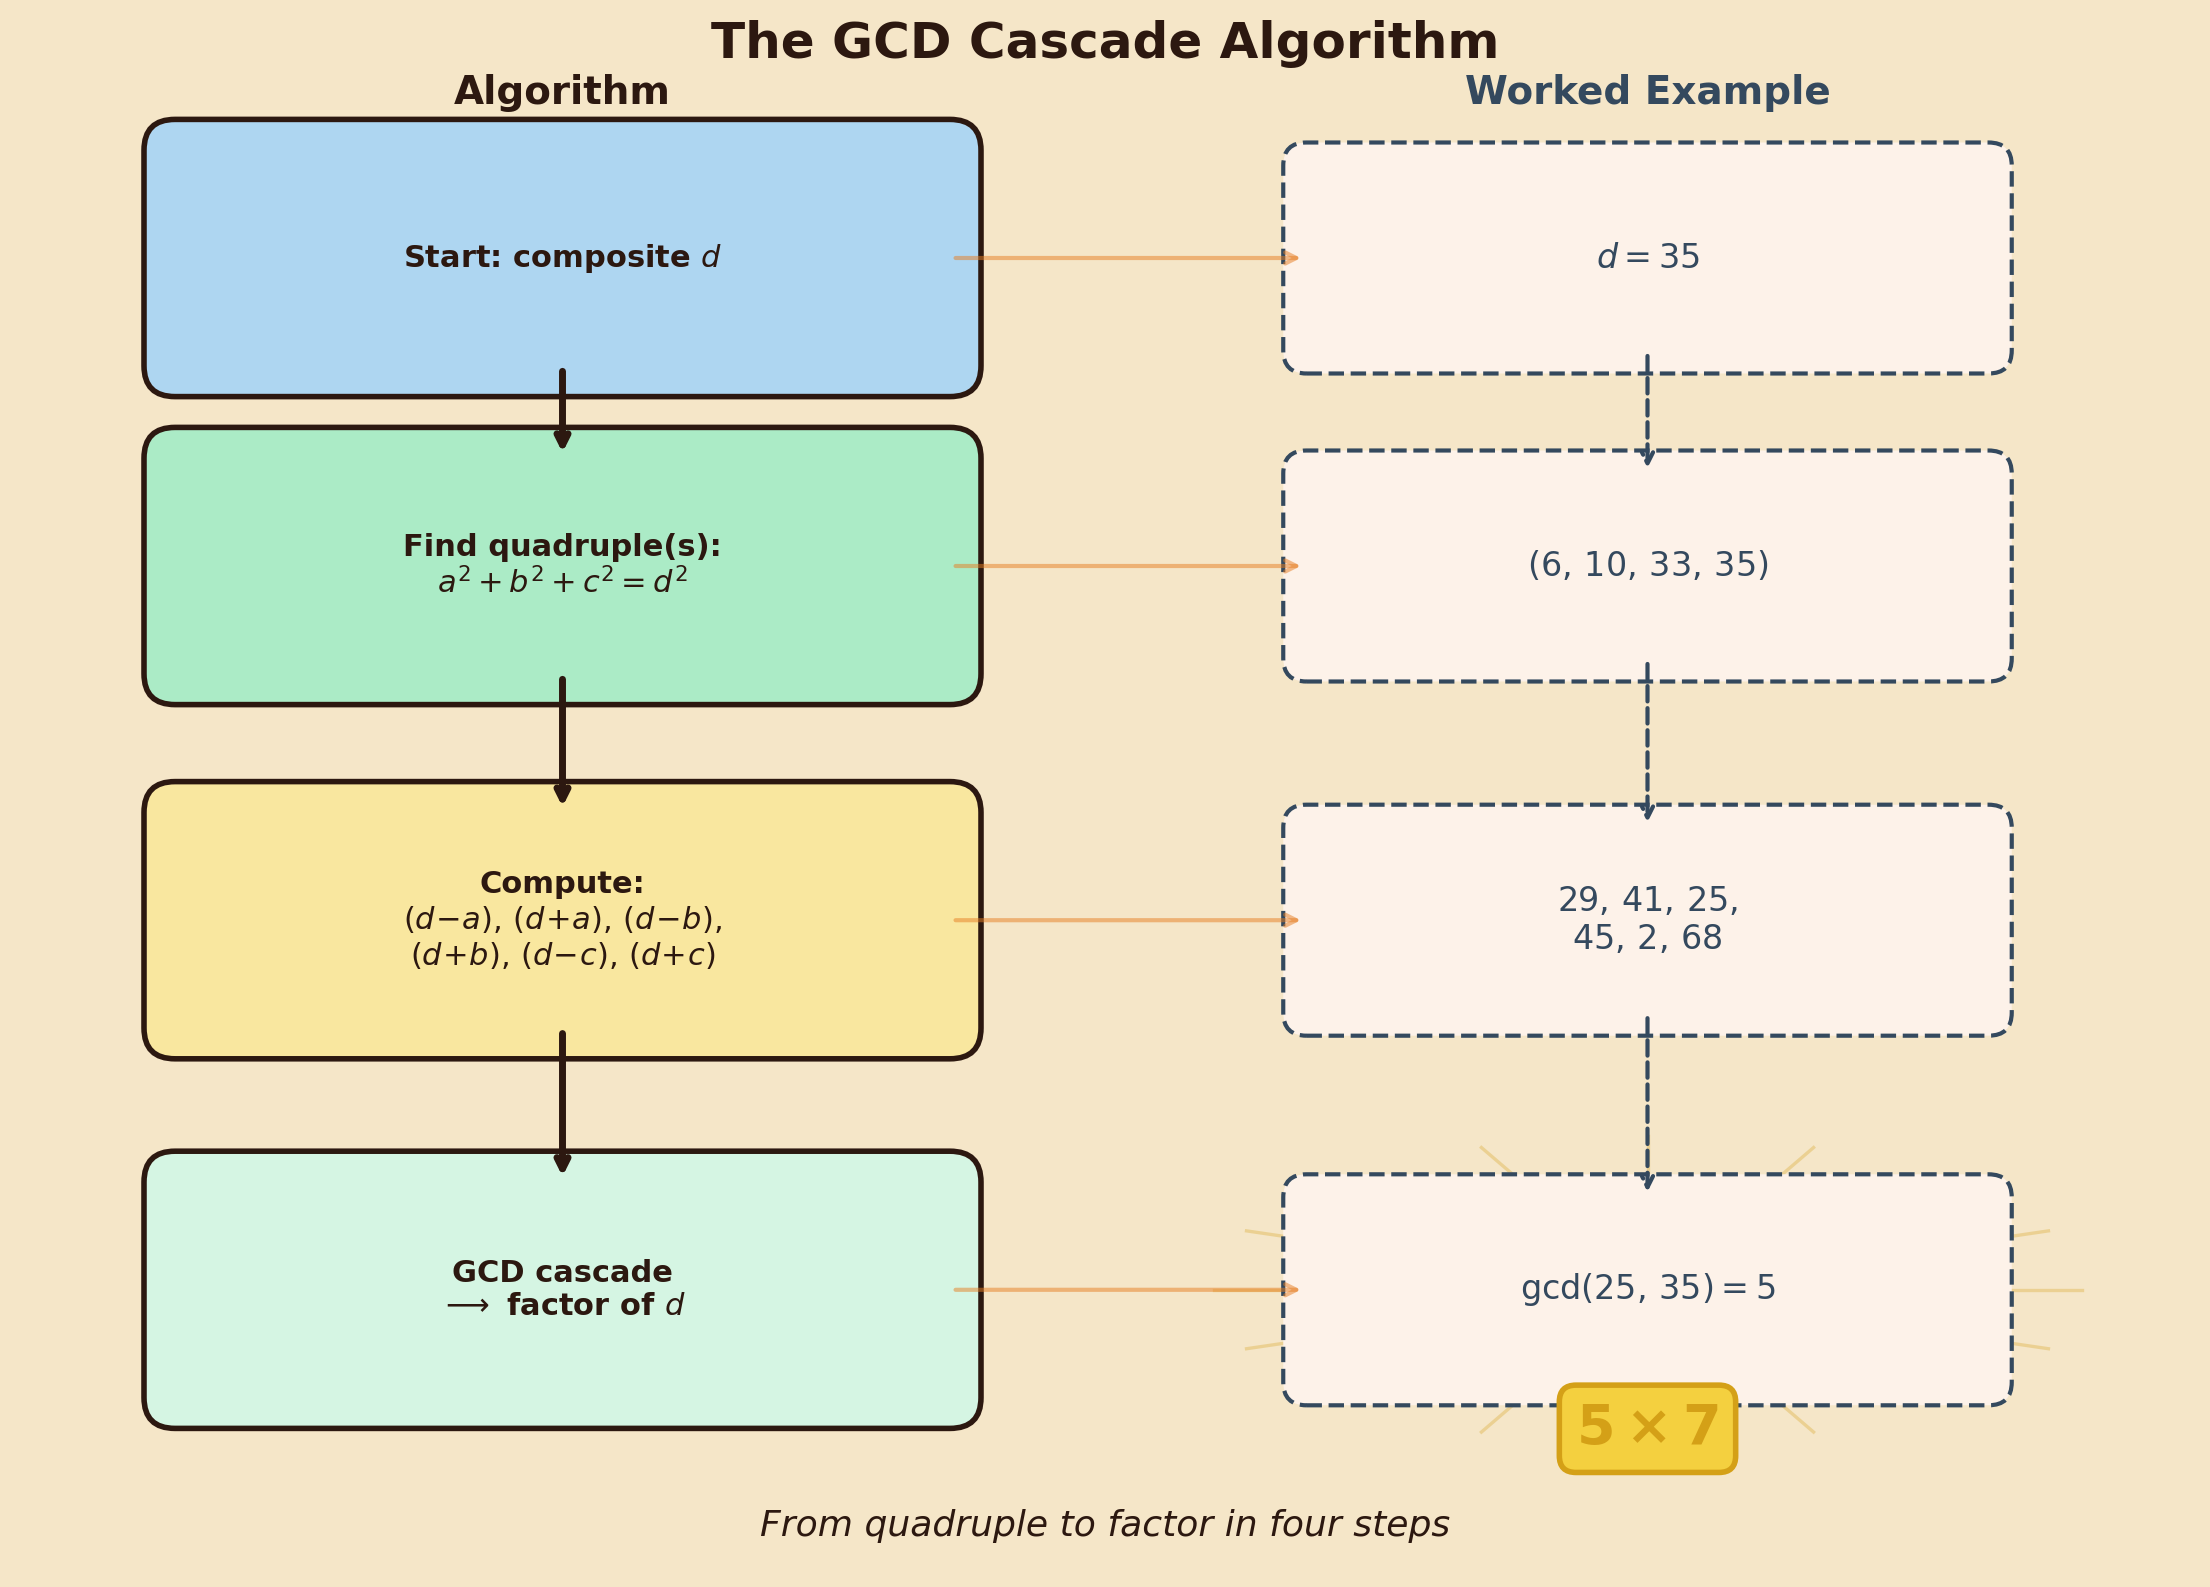
\includegraphics[width=0.82\textwidth]{../Chapter13/images/fig14_gcd_flowchart.png}
\caption{A flowchart with four rounded boxes connected by arrows. Box 1: "Start: composite $d$." Box 2: "Find quadruple(s): $a^2 + b^2 + c^2 = d^2$." Box 3: "Compute small factors:\ldots}
\end{figure}


\bigskip


The Pythagorean quadruple is not merely a higher-dimensional curiosity, a four-variable generalization filed away in some dusty corner of number theory. It is a \textit{factoring instrument} --- a machine whose moving parts are channels, cascades, and the gears of the GCD. Every quadruple dissects its hypotenuse into small factors, each one a potential trapdoor. Every pair of quadruples sharing a hypotenuse generates a web of divisibility constraints that no composite can survive. Brahmagupta's identity supplies the algebraic muscle. Euclid's lemma supplies the logical scalpel. And the ancient method of descent supplies the recursion that strips factors away, one layer at a time, until the prime core is exposed.

The eavesdropper's puzzle from our opening paragraph? The quadruple $(390, 1{,}738, 4{,}122, 4{,}579)$ yields $d - c = 4{,}579 - 4{,}122 = 457$, and $\gcd(457, 4{,}579) = 457$. So $4{,}579 = 457 \times \ldots$ well, let the reader finish the division. The safe is open.

